\chapter{Multidimensional Vectors}
\section{Vectors Space}

In this section we
introduce an algebraic structure for $\bbR^n$,  the vector space in $n$-dimensions. 

We assume that you are familiar with the geometric
interpretation of members of $\bbR^2$ and $\bbR^3$ as the
rectangular coordinates of
points in a plane and three-dimensional space, respectively. 

Although $\bbR^n$ cannot be visualized geometrically if $n\ge4$, geometric
ideas from $\bbR$, $\bbR^2$, and $\bbR^3$ often help us to
interpret the properties of $\bbR^n$ for arbitrary $n$.

\begin{df}
The $n$-dimensional space, $\reals^n$, is defined as the set
$$ \reals^n = \left\{ \left(x_1, x_2, \dots , x_n\right): x_k \in \reals\right\}. $$
\end{df}

Elements $\vector{v} \in \bbR^n$ will be called \negrito{vectors} and will be written in boldface  $\vector{v} $. In the blackboard the
vectors generally are written with an arrow $\vec{v}$.

\begin{df}
If $\vector{x}$ and $\vector{y}$ are two vectors in $\reals^n$ their
\negrito{vector sum} $\vector{x} + \vector{y}$ is defined by the
coordinatewise addition
\begin{equation}\vector{x} + \vector{y} = \left(x_1 + y_1, x_2 + y_2,  \dots, x_n + y_n \right).    \label{eq:vector_addition}\end{equation}
\end{df}


Note that the symbol ``$+$'' has two distinct meanings in \eqref{eq:vector_addition}: on the
left, ``$+$'' stands for the newly defined addition of members of
$\bbR^n$ and, on the right, for the usual addition of real numbers.


The vector with all components $0$ is called the \negrito{zero vector} and is denoted by $\mathbf{0}$. It has
the property that $\vector{v} + \mathbf{0} = \vector{v}$ for every vector $\vector{v}$; in other words, $\mathbf{0}$ is the identity element
for vector addition. 

\begin{df}A real number $\lambda\in\reals$ will be called a \negrito{scalar}.
If $\lambda\in\reals$ and $\vector{x}\in\reals^n$ we define \negrito{
scalar multiplication} of a vector and a scalar by   the
coordinatewise multiplication \begin{equation}\lambda\vector{x} = \left(\lambda x_1, \lambda  x_2,
\dots, \lambda x_n \right).
\label{eq:scalar_multiplication}\end{equation}
\end{df}


The space $\reals^n$ with the operations of sum and scalar multiplication defined above will be called $n$ dimensional vector space.

The vector $(-1)\vector{x}$ is also denoted by $-\vector{x}$ and is called the \negrito{negative} or \negrito{opposite}
of $\vector{x}$

We leave the proof of the following theorem to the reader
\begin{thm}\label{thmtype:5.1.2}
If $\vector{x},$ $\vector{z},$ and $\vector{y}$ are in $\bbR^n$
and
$\lambda, \lambda_1$ and $\lambda_2$ are real numbers$,$ then
\begin{dingautolist}{202}
\item % (a)
 $\vector{x}+\vector{z}=\vector{z}+\vector{x}$  $($vector addition
is commutative$).$
\item % (b)
$(\vector{x}+\vector{z})+\vector{y}=\vector{x}+(\vector{z}+\vector{y})$
$($vector addition is associative$).$
\item % (c)
 There is a unique vector $\mathbf{0},$ called the zero vector$,$
such that $\vector{x}+\mathbf{0}=\vector{x}$ for all $\vector{x}$ in
$\bbR^n.$
\item % (d)
 For each $\vector{x}$ in $\bbR^n$ there is a unique vector
$-\vector{x}$ such that $\vector{x}+(-\vector{x})=\mathbf{0}.$
\item % (e)
 $\lambda_1(\lambda_2\vector{x})=(\lambda_1 \lambda_2)\vector{x}.$
\item % (f)
$(\lambda_1+\lambda_2)\vector{x}=\lambda_1\vector{x}+\lambda_2\vector{x}.$
\item % (g)
 $\lambda(\vector{x}+\vector{z})=\lambda\vector{x}+\lambda\vector{z}.$
\item % (h)
 $1\vector{x}=\vector{x}.$
\end{dingautolist}
\end{thm}

Clearly, $\mathbf{0}=(0,0, \dots,0)$ and, if
$\vector{x}=(x_1,x_2, \dots,x_n)$, then
$$
-\vector{x}=
(-x_1,-x_2, \dots,-x_n).
$$

We  write $\vector{x}+(-\vector{z})$  as
$\vector{x}-\vector{z}$. The vector $\mathbf{0}$ is called the \negrito{origin\/}.



In a more general context, a nonempty set $V$,
together with
two operations  $+,\cdot$ is
said to be a \negrito{vector space} if it has the
properties listed
in Theorem~\ref{thmtype:5.1.2}. The members of a vector space are called
\negrito{vectors}.



When we wish to note that we  are
regarding a
member of $\bbR^n$ as part of this algebraic structure, we will
speak of it as a vector; otherwise, we will speak of it as a point. 


\begin{df}
The \negrito{canonical ordered basis} for $\reals^n$ is the collection of
vectors
$$\{\vector{e}_1, \vector{e}_2,\ldots,
\vector{e}_n,\}$$ with
$$ \vector{e}_k = \underbrace{\left(0,  \dots,  1, \dots,  0\right)}_{
\text{a $1$
in the $k$ slot and $0$'s everywhere else}}.$$ 
\end{df}

Observe that \begin{equation}
               \sum _{k = 1} ^n v_k\vector{e}_k   =  \left(v_1,
v_2, \dots, v_n\right). \label{eq:span2}
             \end{equation}
             
This means that any vector can be written as sums of scalar multiples   of the standard basis. We will discuss this fact more deeply in the next section.           


\begin{df}
Let $\point{a}, \point{b}$ be distinct points in $\reals^n$ and let $\vector{x}=\point{b}-\point{a}\neq
\vector{0}$,. The \negrito{parametric line}
passing through $\point{a}$ in the direction of $\vector{x}$ is the
set
$$ \left\{\point{r}\in\reals^n:\point{r}=\point{a}+t\vector{x} \right\}. $$
\end{df}

% The  vector $\vector{x}$ in $\reals^n$ is called the 


\begin{exa}
Find the parametric equation of the line passing through the points $(1, 2, 3)$ and  $\left(-2, -1, 0\right)$.
\end{exa}
\begin{solu} The line follows the direction $$ \left(1 - (-2), 2 - (-1), 3 - 0\right) = \left(3, 3, 3\right).
$$ The desired equation is $$\left(x, y,  z\right) =  \left(1, 2, 3\right) + t\left(3, 3,  3\right).   $$

Equivalently 
$$\left(x, y,  z\right) =  \left(-2, -1, 2\right) + t\left(3, 3,  3\right).   $$
\end{solu}


\subsection*{Length, Distance, and Inner Product}

\begin{df}
Given vectors $\vector{x}, \vector{y} $ of $\reals^n$, their \negrito{inner product} or \negrito{
dot product} is defined as $$ \dotprod{x}{y}  = \sum _{k=1} ^n x_ky_k.$$
\end{df}

\begin{thm}
 For  $\vector{x}, \vector{y},  \vector{z} \in \reals^n$, and $\alpha$ and $\beta$ real numbers, we have>
\begin{dingautolist}{202}
 \item $(\alpha \vector{x}+\beta \vector{y}) \bp \vector{z}= \alpha (\vector{x}\bp \vector{z})+\beta  (\vector{y}\bp \vector{z})$
 \item $\vector{x}\bp \vector{y}= \vector{y} \bp \vector{x}$
 \item $\vector{x}\bp \vector{x}\geq 0$
 \item $\vector{x}\bp \vector{x}= 0$ if and only if $\vector{x}=\vector{0}$
\end{dingautolist}

\end{thm}

The proof of this theorem is simple and will be left as exercise for the reader.

The \negrito{norm} or \negrito{length} of a vector $\vector{x}$, denoted as $\norm{\vector{x}}$, is defined as 
\[\norm{\vector{x}}=\sqrt{ \dotprod{x}{x}} \]

\begin{df}
 Given vectors $\vector{x}, \vector{y} $ of $\reals^n$, their \negrito{
distance} is 
\[d(\vector{x},\vector{y})=\norm{\vector{x}-\vector{y}}=\sqrt{\dotprod{(x-y)}{
(x-y)}}=\sum_{i=1}^n \left(x_i-y_i \right)^2\]
\label{def:lenght}
\end{df}

If $n=1$, the previous definition of length  reduces to the familiar absolute
value, for $n=2$ and $n=3$, the length
and distance of Definition~\ref{def:lenght} reduce to the familiar
definitions for the two and three dimensional space.
\begin{df} A vector  $\vector{x}$  is  called \negrito{unit vector}
 \[ \norm{\vector{x}}=1.\]
\end{df}



\begin{df} Let $\vector{x}$ be  a non-zero vector, then the associated 
  \negrito{versor} (or normalized vector)  denoted $\hat {\vector{x}}$  is the unit vector 
 \[ \hat{\vector{x}}=\dfrac{\vector{x}}{\norm{\vector{x}}}.\]
\end{df}




We now establish one of the most useful inequalities in analysis.
\begin{thm}[Cauchy-Bunyakovsky-Schwarz Inequality] Let
$\vector{x}$ and $\vector{y}$  be any two vectors in $\reals^n$.
Then we have
$$
 |\dotprod{x}{y}| \leq \norm{\vector{x}}\norm{\vector{y}} .$$\label{thm:cauchy_schwarz}
\end{thm}
\begin{proof}
Since the norm of any vector is non-negative, we have $$
\begin{array}{lll} \norm{\vector{x} + t\vector{y}} \geq 0 & \iff &
(\vector{x} + t\vector{y})\bp (\vector{x} +t\vector{y}) \geq 0 \\ &
\iff & \dotprod{x}{x} + 2t\dotprod{x}{y} + t^2\dotprod{y}{y} \geq 0
\\ & \iff & \norm{\vector{x}}^2 + 2t\dotprod{x}{y} +
t^2\norm{\vector{y}}^2 \geq 0.
\end{array}$$ This last expression is a quadratic polynomial in
$t$ which is always non-negative. As such its discriminant must be
non-positive, that is, $$ (2\dotprod{x}{y})^2 -
4(\norm{\vector{x}}^2)(\norm{\vector{y}}^2) \leq 0 \iff
|\dotprod{x}{y}| \leq \norm{\vector{x}}\norm{\vector{y}} ,
$$giving the theorem.
\end{proof}


The Cauchy-Bunyakovsky-Schwarz inequality can be written as
\begin{equation} \left|\sum _{k = 1} ^n x_k y_k \right| \leq
\left(\sum _{k = 1} ^nx_k ^2\right)^{1/2} \left(\sum _{k = 1} ^ny_k
^2\right)^{1/2}, \label{eq:cbs_sum_form}\end{equation} for real
numbers $x_k, y_k$.


\begin{thm}[Triangle Inequality] Let
$\vector{x}$ and $\vector{y}$ be  any two vectors in $\reals^n$.
Then we have
$$\norm{\vector{x} + \vector{y}} \leq \norm{\vector{x}} + \norm{\vector{y}}.$$
\label{defdesitriangular}
\end{thm}
\begin{proof}
$$\begin{array}{lll}
||\vector{x} + \vector{y}||^2 & = & (\vector{x} + \vector{y})\bp (\vector{x} + \vector{y}) \\
& = & \vector{x}\bp\vector{x} + 2\vector{x}\bp\vector{y} +
\vector{y}\bp\vector{y} \\
& \leq & ||\vector{x}||^2  + 2||\vector{x}||||\vector{y}|| +
||\vector{y}||^2 \\
& = & (||\vector{x}|| + ||\vector{y}||)^2,
\end{array}$$from where the desired result follows.
\end{proof}

\begin{corollary}\label{defdesitriangular2}
 If $\mathbf{x},$ $\mathbf{y},$ and
$\mathbf{z}$ are  in $\bbR^n,$ then
$$
|\mathbf{x}-\mathbf{y}|\le
|\mathbf{x}-\mathbf{z}|+|\mathbf{z}-\mathbf{y}|.
$$
\end{corollary}

\begin{proof} Write
$$
\mathbf{x}-\mathbf{y}=(\mathbf{x}-\mathbf{z})+(\mathbf{z}-\mathbf{y}),
$$
and apply Theorem~\ref{defdesitriangular}.
\end{proof}



\begin{df}
Let $\vector{x}$ and $\vector{y}$ be two non-zero vectors  in $\reals^n$. Then the angle
$\anglebetween{x}{y}$ between them is given by the relation $$\cos
\anglebetween{x}{y} =
\dfrac{\dotprod{x}{y}}{\norm{\vector{x}}\norm{\vector{y}}}.
$$This expression agrees with the geometry in the case of the dot
product for $\reals^2$ and $\reals^3$.
\end{df}



\begin{df}
 Let $\vector{x}$ and $\vector{y}$ be two non-zero vectors  in $\reals^n$. This vectors  are said  orthogonal if the angle between them is 90 degrees.  Equivalently, if:
 $\vector{x} \bp \vector{y}=0$ 
\end{df}



% \begin{exa}
% Assume that $a_k, b_k, c_k, k = 1, \ldots, n$, are positive real
% numbers. Shew that
% $$\left(\sum _{k = 1} ^n a_kb_kc_k\right)^{4}
% \leq \left(\sum _{k = 1} ^n a_k ^4\right)\left(\sum _{k = 1} ^n b_k
% ^4\right) \left(\sum _{k = 1} ^n c_k ^2\right)^{2}.$$\end{exa}
% \begin{solu}Using CBS on $\sum _{k = 1} ^n (a_kb_k)c_k$ once we obtain
% $$\sum _{k = 1} ^n a_kb_kc_k
% \leq \left(\sum _{k = 1} ^n a_k ^2b_k ^2\right)^{1/2} \left(\sum _{k
% = 1} ^n c_k ^2\right)^{1/2}.
% $$Using CBS again on $\left(\sum _{k = 1} ^n a_k ^2b_k ^2\right)^{1/2}$ we obtain
% $$
% \begin{array}{lll}
% \sum _{k = 1} ^n a_kb_kc_k  & \leq &
%  \left(\sum _{k = 1} ^n a_k ^2 b_k ^2\right)^{1/2}
% \left(\sum _{k = 1} ^n c_k ^2\right)^{1/2} \\
%   & \leq & \left(\sum _{k = 1} ^n a_k ^4\right)^{1/4}
% \left(\sum _{k = 1} ^n b_k ^4\right)^{1/4}
% \left(\sum _{k = 1} ^n c_k ^2\right)^{1/2}, \\
% \end{array}
% $$which gives the required inequality.
% \end{solu}






Let  $P_0 = (p_1, p_2, \dots, p_n)$, and  $\vector{n} = (n_1, n_2,\dots ,n_n)$
be a nonzero vector. 

\begin{df}
The hyperplane defined by the point $P_0$ and the vector $\vector{n}$ is defined as the set of points 
$P:(x_1, , x_2,\dots ,x_n)\in \bbR^n$,  
such that the vector drawn from $P_0$ to $P$ is perpendicular to  $\vector{n}$.
\[\displaystyle \vector{n} \bp (\vector{P} -\vector{P} _{0})=0.\]
\end{df}


Recalling that two vectors are perpendicular if and only if their dot product is
zero, it follows that the desired hyperplane can be described as the set of all points $P$ such that

\[\displaystyle \vector{n} \bp (\vector{P} -\vector{P} _{0})=0.\]
 Expanded this becomes

\[\displaystyle n_1(x_1-p_1)+n_2(x_2-p_2)+\cdots+n_n(x_n-p_n)=0,\] 
which is the point-normal form of the equation of a hyperplane. This is just a linear equation

\[\displaystyle n_1x_1+n_2x_2+\cdots n_nx_n+d=0,\] 
where

\[\displaystyle d=-(n_1p_1+n_2p_2+\cdots + n_np_{n}).\]
% Conversely, it is easily shown that if a, b, c and d are constants and a, b, and c are not all zero, then the graph of the equation
% 
% {\displaystyle ax+by+cz+d=0,} 
% is a plane having the vector n = (a, b, c) as a normal.[2] This familiar equation for a plane is called the general form of the equation of the plane.[3]
% 


% 
% We now use the CBS inequality to establish another important
% inequality. We need some preparatory work.
% \begin{lem}\label{lem:for-AMGM}Let $a_k>0$, $q_k>0$, with $\sum _{k=1} ^n q_k =
% 1$. Then $$ \lim _{x\to 0} \log\left(\sum _{k=1} ^n q_ka_k
% ^x\right)^{1/x} = \sum _{k=1} ^n q_k\log a_k.
% $$
% \end{lem}
% \begin{proof}
% Recall that $\log (1+x) \sim x$ as $x\to 0$. Thus
% $$\begin{array}{lll} \lim _{x\to 0} \log\left(\sum _{k=1} ^n q_ka_k
% ^x\right)^{1/x} & = & \lim _{x\to
% 0} \dfrac{\log\left(\sum _{k=1} ^n q_ka_k ^x\right)}{x}\\
% & = &  \lim _{x\to
% 0} \dfrac{\sum _{k=1} ^n q_k(a_k ^x-1)}{x}\\
% & = &  \lim _{x\to
% 0} \sum _{k=1} ^n q_k\dfrac{(a_k ^x-1)}{x}\\
% & = & \sum _{k=1} ^n q_k\log a_k.
% \end{array}$$
% \end{proof}
% \begin{thm}[Arithmetic Mean-Geometric Mean Inequality]\label{thm:arith_geom_meanbyCBS} Let $a_k\geq 0$. Then
% $$ \sqrt[n]{a_1a_2\cdots a_n}  \leq \dfrac{a_1+a_2+\cdot + a_n}{n}. $$
% \end{thm}
% \begin{proof}
% If $b_k \geq 0$, then by CBS
% \begin{equation}
% \dfrac{1}{n}\sum _{k=1} ^n b_k \geq \left(\dfrac{1}{n}\sum _{k=1} ^n
% \sqrt{b_k} \right)^2. \label{eq:cons-of-CBS}
% \end{equation}
% Successive applications of (\ref{eq:cons-of-CBS}) yield the monotone
% decreasing sequence
% $$ \dfrac{1}{n}\sum _{k=1} ^n a_k \geq \left(\dfrac{1}{n}\sum _{k=1} ^n
% \sqrt{a_k} \right)^2 \geq \left(\dfrac{1}{n}\sum _{k=1} ^n
% \sqrt[4]{a_k} \right)^4 \geq \ldots , $$ which by Lemma
% \ref{lem:for-AMGM} has limit
% $$\exp \left(\dfrac{1}{n}\sum _{k=1} ^n \log a_k \right) = \sqrt[n]{a_1a_2\cdots a_n},  $$
% giving
% $$ \sqrt[n]{a_1a_2\cdots a_n}  \leq \dfrac{a_1+a_2+\cdot + a_n}{n}, $$
% as wanted.
% \end{proof}
% 
% \begin{exa} For any positive integer $n
% > 1$ we have
% $$1\cdot 3 \cdot 5 \cdots \cdot (2n - 1) < n^n.$$ For, by AMGM,
% $$1\cdot 3 \cdot 5 \cdots \cdot (2n - 1) < \left(\dfrac{1 +  3 + 5 + \cdots + (2n -
% 1)}{n}\right)^n = \left(\dfrac{n^2}{n}\right)^n = n^n.$$Notice that
% since the factors are unequal we have strict inequality.
% \end{exa}
% \begin{df}
%  Let $x_1 > 0, x_2 > 0, \ldots , x_n >
% 0$. Their \negrito{harmonic mean} is given by
% $$\dfrac{n}{
% \dfrac{1}{a_1} + \dfrac{1}{a_2} + \cdots + \dfrac{1}{a_n}}.
% $$
% \end{df}
% As a corollary to AMGM we obtain
% \begin{cor}[Harmonic Mean-Geometric Mean Inequality] Let $y_1> 0, y_2 > 0, \ldots , y_n >
% 0$. Then
% $$\dfrac{n}{
% \dfrac{1}{b_1} + \dfrac{1}{b_2} + \cdots + \dfrac{1}{y_n }} \leq
% (b_1b_2\cdots y_n )^{1/n}.$$ \label{cor:harm_geom_mean}
% \end{cor}
% \begin{proof}
% This follows by putting $a_k = \dfrac{1}{b_k}$ in Theorem
% \ref{thm:arith_geom_meanbyCBS} . For then $$
% \left(\dfrac{1}{b_1}\dfrac{1}{b_2}\cdots\dfrac{1}{y_n }\right)^{1/n}
% \leq \dfrac{\dfrac{1}{b_1} + \dfrac{1}{b_2} + \cdots +
% \dfrac{1}{y_n }}{n}.
% $$
% \end{proof}
% Combining Theorem \ref{thm:arith_geom_meanbyCBS}  and Corollary
% \ref{cor:harm_geom_mean}, we deduce \begin{cor}[Harmonic
% Mean-Arithmetic Mean Inequality] \label{cor:harm_arith_mean} Let
% $y_1> 0, y_2 > 0, \ldots , y_n > 0$. Then
% $$\dfrac{n}{
% \dfrac{1}{b_1} + \dfrac{1}{b_2} + \cdots + \dfrac{1}{y_n }} \leq
% \dfrac{b_1+b_2+\cdots + y_n }{n}.$$
% 
% \end{cor}
% \begin{exa}
% Let $a_k > 0,$ and $s = x_1 + x_2 + \cdots + a_n$. Prove that
% $$\sum _{k = 1} ^n \dfrac{s}{s -
% a_k} \geq  \dfrac{n^2}{n - 1}$$and
% $$\sum _{k = 1} ^n \dfrac{a_k}{s - a_k} \geq  \dfrac{n}{n - 1}.$$
% \end{exa}
% \begin{solu}  Put $b_k = \dfrac{s}{s - a_k}$. Then $$ \sum _{k = 1} ^n
% \dfrac{1}{b_k} = \sum _{k = 1} ^n \dfrac{s - a_k}{s} = n - 1
% $$ and from Corollary
% \ref{cor:harm_arith_mean},
% $$ \dfrac{n}{n - 1}  \leq \dfrac{\sum _{k = 1} ^n \dfrac{s}{s -
% a_k}}{n},
% $$from where the first inequality is proved.
% 
% \bigskip
% 
% Since $\dfrac{s}{s - a_k}  - 1 = \dfrac{a_k}{s - a_k},$ we have
% $$\begin{array}{lll}\sum _{k = 1} ^n \dfrac{a_k}{s - a_k} & = &
% \sum _{k = 1} ^n \left(\dfrac{s}{s - a_k}  - 1\right) \\
% & = & \sum _{k = 1} ^n \left(\dfrac{s}{s - a_k}\right) - n \\
% & \geq &   \dfrac{n^2}{n - 1} - n \\
% & = & \dfrac{n}{n - 1}.\end{array}$$
% \end{solu}
% 
% \bigskip
% 
% \section*{\psframebox{Exercises}}
% \begin{multicols}{2}\columnseprule 1pt \columnsep 25pt\multicoltolerance=900
% 
% \bigskip
% 
% \begin{problem}
% The \negrito{Arithmetic Mean Geometric Mean Inequality} says that if
% $a_k \geq 0$ then $$(a_1a_2\cdots a_n)^{1/n} \leq \dfrac{x_1 + x_2 +
% \cdots + a_n}{n}. $$ Equality occurs if and only if $x_1 = x_2 =
% \ldots = a_n.$ In this exercise you will follow the steps of a proof
% by George P\'{o}lya.
% \begin{enumerate}
% \item Prove that $\forall x\in\reals , \  x \leq e^{x - 1}.$
% \item Put $$A_k = \dfrac{na_k}{x_1 + x_2 + \cdots + a_n},$$ and $G_n =
% a_1a_2\cdots a_n$. Prove that $$A_1A_2\cdots A_n =
% \dfrac{n^nG_n}{(x_1 + x_2 + \cdots + x_n )^n},$$ and that
% $$A_1 + A_2 + \cdots + A_n = n.$$
% \item Deduce that
% $$G_n \leq \left(\dfrac{x_1 + x_2 + \cdots +
% a_n}{n}\right)^n.$$
% \item Prove the AMGM inequality by assembling the results above.
% \end{enumerate}
% \begin{answer}\noindent
% \begin{enumerate}
% \item Put $f:\reals \rightarrow \reals$, $f(x) = e^{x - 1} - x.$ Clearly $f(1)
% = e^0 - 1 = 0$. Now,
% $$f'(x) = e^{x - 1} - 1,$$
% $$f''(x) = e^{x - 1}.$$
% If $f'(x) = 0$ then $e^{x - 1} = 1$ implying that $x = 1$. Thus $f$
% has a single minimum point at $x = 1$. Thus for all real numbers $x$
% $$ 0 = f(1) \leq f(x) = e^{x - 1} - x,$$which gives the desired
% result.
% \item Easy Algebra!
% \item Easy Algebra!
% \item By the preceding results, we have
% $$A_1 \leq \exp (A_1 - 1),$$
% $$A_2 \leq \exp (A_2 - 1),$$
% $$\dots$$
% $$A_n \leq \exp (A_n - 1).$$Since all the quantities involved are
% non-negative, we may multiply all these inequalities together, to
% obtain,
% $$A_1A_2\cdots A_n \leq \exp (A_1 + A_2 + \cdots + A_n - n).$$In
% view of the observations above, the preceding inequality is
% equivalent to
% $$\dfrac{n^nG_n}{(x_1 + x_2 + \cdots + x_n )^n} \leq \exp (n - n) = e^0 =
% 1.$$We deduce that
% $$G_n \leq \left(\dfrac{x_1 + x_2 + \cdots +
% a_n}{n}\right)^n,$$which is equivalent to
% $$(a_1a_2\cdots a_n)^{1/n} \leq \dfrac{x_1 + x_2 + \cdots + a_n}{n}. $$
% Now, for equality to occur, we need each of the inequalities $A_k
% \leq \exp (A_k - 1)$ to hold. This occurs, in view of the preceding
% lemma, if and only if $A_k = 1, \ \forall k$, which translates into
% $x_1 = x_2 = \ldots = a_n$. This completes the proof.
% 
% \end{enumerate}
% 
% 
% \end{answer}
% 
% \end{problem}
% \begin{problem}
% Demonstrate that if   $x_{1},x_{2}, \ldots ,x_{n},$  are strictly
% positive real numbers then
% $$\left(x_{1}+x_{2}+ \ldots +x_{n}\right)\left(\dfrac{1}{x_{1}}+\dfrac{1}{x_{2}}+ \ldots +\dfrac{1}{x_{n}}%
% \right)\geq n^{2}.$$
% \begin{answer}By CBS,
% $$\begin{array}{lll}\left(x_{1}+x_{2}+ \ldots +x_{n}\right)\left(\dfrac{1}{x_{1}}+\dfrac{1}{x_{2}}+ \ldots +\dfrac{1}{x_{n}}%
% \right)& \geq &  \left(\stackunder{i=1}{\stackrel{n}{\sum }}\sqrt{x_{i}}\dfrac{1}{\sqrt{x_{i}}%
% }\right)^{2} \\
% & = & n^2.\end{array}$$
% 
% \end{answer}
% \end{problem}
% \begin{problem}[USAMO 1978]
% Let $a,b,c,d,e$ be real numbers such that
% $$a+b+c+d+e=8, \qquad a^{2}+b^{2}+c^{2}+d^{2}+e^{2}=16.$$Maximise the value of  $e$.
% 
% \begin{answer}
% By CBS, $$\begin{array}{lll}\left(a+b+c+d\right)^{2}\leq
% \left(1+1+1+1\right)\left(a^{2}+b^{2}+c^{2}+d^{2}\right) & = &
% 4\left(a^{2}+b^{2}+c^{2}+d^{2}\right).\end{array}$$ Hence,
% $$\left(8-e\right)^{2}\leq 4\left(16-e^{2}\right)\iff
% e\left(5e-16\right)\leq 0\iff 0\leq e\leq \dfrac{16}{5}.$$ The
% maximum value $e=\dfrac{16}{5}$ is reached when
% $a=b=c=d=\dfrac{6}{5}.$
% 
% \end{answer}
% \end{problem}
% 
% \begin{problem} Find all positive real numbers  $$a_1\leq a_2\leq \ldots \leq a_n
% $$ such that
% $$\sum _{k=1} ^n a_k =96, \qquad \sum _{k=1} ^n a_k ^2 =144, \qquad \sum _{k=1} ^n a_k ^3 =216.  $$
% \begin{answer}
% Observe that  $96\cdot 216=144^2$ and by CBS,
% $$  \sum _{k=1} ^n a_k ^2  \leq \left( \sum _{k=1} ^n a_k ^3 \right)\left( \sum _{k=1} ^n a_k \right).  $$
% As there is equality, $$ (a_1, a_2, \ldots , a_n) = t (x_1 ^3, a_2
% ^3, \ldots , a_n^3)$$for some real number $t$. Hence $x_1 = x_2 =
% \ldots = a_n=a$, from where $na=96$, $na^2=144$ gives
% $a=\dfrac{3}{2}$ y $n=32$.
% \end{answer}
% \end{problem}
% 
% \begin{problem}
% Demonstrate that for integer $n>1$ we have, $$
% n!<\left(\dfrac{n+1}{2}\right)^n.
% $$
% \begin{answer}
% Applying the AM-GM inequality, for $1,2,\ldots , n$:
% $$ n!^{1/n}= (1\cdot 2 \cdots n)^{1/n}< \dfrac{1+2+\cdots + n}{n} = \dfrac{n+1}{2},
% $$with strict inequality for
% $n>1$.
% \end{answer}
% \end{problem}
% 
% 
% \begin{problem} Let $f(x) = (a + x)^5(a - x)^3, \ x\in
% [-a; a].$ Find the maximum value of de  $f$ using the AM-GM
% inequality.
% \begin{answer}If $x\in [-a; a]$, then $a + x \geq 0$ and $a - x \geq 0$, and thus we may use AM-GM with  $n = 8$,
% $x_1 = x_2 = \cdots = a_5 = \dfrac{a + x}{5}$ and $a_6 = a_7 = a_8 =
% \dfrac{a - x}{3}.$ We deduce that
% $$\left(\dfrac{a + x}{5}\right)^5 \left(\dfrac{a - x}{3}\right)^3 \leq \left(\dfrac{5\left(\dfrac{a + x}{5}\right) + 3\left(\dfrac{a - x}{3}\right) }{8}\right)^8
%  = \left(\dfrac{a}{4}\right)^8, $$
% from where
% $$f(x) \leq \dfrac{5^53^3a^8}{4^8},$$with equality if and only if
% $\dfrac{a + x}{5} = \dfrac{a - x}{3}$. \end{answer}
% \end{problem}
% 
% 
% \begin{problem}Prove that the sequence \mbox{$x_n = \left(1 + \dfrac{1}{n}\right)^{n}$}, $n = 1,
% 2, \ldots$ is strictly increasing. \begin{answer} Applying AM-GM to
% the set of  $n + 1$ numbers
% $$1, 1 +
% \dfrac{1}{n}, 1 + \dfrac{1}{n}, \ldots , 1 + \dfrac{1}{n},$$has
% arithmetic mean
% $$1 + \dfrac{1}{n + 1}$$ and geometric mean
% $$\left(1 +
% \dfrac{1}{n}\right)^{n/(n + 1)}.$$Therefore,
% $$1 +
% \dfrac{1}{n + 1} >  \left(1 + \dfrac{1}{n}\right)^{n/(n + 1)},$$
% that is
% $$\left(1 +
% \dfrac{1}{n + 1}\right)^{n + 1} >  \left(1 +
% \dfrac{1}{n}\right)^{n},$$ which means
% $$x_{n + 1} > x_n,$$giving the assertion.
% \end{answer}
% \end{problem}
% 
% \end{multicols}
% 
% 




\section{Basis and Change of Basis}

\subsection{Linear Independence and Spanning Sets}
\begin{df}
Let $\lambda_i \in \bbR, 1\leq i\leq n$. Then
the vectorial sum
$$\sum_{j = 1} ^n \lambda_j\vector{ x}_j$$ is said to be a \negrito{linear
combination} of the vectors  $\vector{ x}_i \in \bbR ^n,  1 \leq i \leq n.$
\end{df}

\begin{df}
The vectors $\vector{ x}_i \in \bbR ^n,  1 \leq i \leq n,$ are \negrito{linearly
dependent} or \negrito{tied} if
$$\exists (\lambda_1, \lambda_2, \cdots , \lambda_n) \in \bbR ^n \setminus \{{\mathbf 0}\} \ \ {\text{ such \ that}\ }
\sum_{j = 1} ^n \lambda_j\vector{ x}_j = \vector{0},$$that is, if there is a
non-trivial linear combination of them adding to the zero vector.
\end{df}\begin{df}
The vectors $\vector{ x}_i \in \bbR ^n,  1 \leq i \leq n,$ are \negrito{linearly
independent} or \negrito{free} if they are not linearly dependent. That
is, if $\lambda_i \in \bbR, 1\leq i \leq n  $
then
$$\sum_{j = 1} ^n \lambda_j\vector{ x}_j = \vector{0} \implies   \lambda_1 = \lambda_2= \cdots = \lambda_n = 0.$$
\end{df}
\begin{rem}
A family of vectors is linearly independent if and only if the
only linear combination of them giving the zero-vector is the
trivial linear combination.
\end{rem}


\begin{exa}

$$\left\{\coord{1 , 2 , 3}, \coord{4 , 5 , 6}, \coord{7 , 8 ,
9}\right\}$$is a tied family of vectors in $\bbR^3$, since
$$(1)\coord{1 , 2 , 3} + (-2) \coord{4 , 5 , 6} + (1)\coord{7 , 8 ,
9} = \coord{0 , 0 , 0}.$$
\end{exa}

\begin{df}
A family of vectors $\{\vector{x}_1, \vector{x}_2, \ldots , \vector{x}_k, \ldots, \}
\subseteq \bbR ^n$ is said to \negrito{span} or \negrito{generate} $\bbR ^n$ if every
$\vector{x}\in \bbR ^n$ can be written as a linear combination of the
$\vector{x}_j$'s. \index{spanning set}           
\end{df}

\begin{exa}
Since  \begin{equation}
               \sum _{k = 1} ^n v_k\vector{e}_k   =  \left(v_1,
v_2, \dots, v_n\right). \label{eq:span2}
             \end{equation}
             
This means that  the canonical basis generate $\bbR ^n$.

\end{exa}


\begin{thm}
If $\{\vector{x}_1, \vector{x}_2, \ldots , \vector{x}_k, \ldots, \} \subseteq \bbR ^n$
spans $\bbR ^n$, then any superset $$\{\vector{y}, \vector{x}_1, \vector{x}_2, \ldots ,
\vector{x}_k, \ldots, \} \subseteq \bbR ^n$$ also spans $\bbR ^n$.
\end{thm}
\begin{proof}
This follows at once from
$$ \sum _{i = 1} ^l \lambda _i \vector{x}_i = 0\vector{y} + \sum _{i = 1} ^l \lambda _i \vector{x}_i.$$
\end{proof}
\begin{exa}
The family of vectors $$\left\{\vector{i} = \coord{1, 0 ,
0}, \vector{j} = \coord{0, 1, 0}, \vector{k} = \coord{0,
0, 1}\right\}$$ spans $\bbR^3$ since given $\coord{a, b,
c}\in\bbR^3$ we may write $$\coord{a, b, c} = a\vector{i} + b\vector{j} +
c\vector{k} .$$ \label{exa:ijk}\end{exa}
\begin{exa}
Prove that the family of vectors $$\left\{\vector{t}_1 = \coord{1, 0 ,
0}, \vector{t}_2 = \coord{1, 1, 0}, \vector{t}_3 = \coord{1,
1, 1}\right\}$$ spans $\bbR^3$.\label{triagbasisr3}\end{exa}
\begin{solu}This follows from the identity
$$\coord{a, b, c} = (a - b)\coord{1, 0, 0} + (b - c)\coord{1, 1, 0} + c\coord{1, 1, 1} = (a - b)\vector{t}_1 + (b - c)\vector{t}_2 + c\vector{t}_3.$$
\end{solu}




\subsection{Basis}
\begin{df}
A family $E=\{\vector{x}_1, \vector{x}_2, \ldots , \vector{x}_k, \ldots\} \subseteq
\bbR ^n$ is said to be a \negrito{basis} of  $\bbR ^n$ if
\begin{dingautolist}{202}
 \item  are linearly
independent,
 \item they span $\bbR ^n$. \index{basis}
\end{dingautolist}
\end{df}
\begin{exa}
The family $$ \vector{e}_i =\left(0 ,\dots , 0, 1,  0, \dots , 0
\right),$$ where there is a $1$ on the $i$-th slot and
$0$'s on the other $n - 1$ positions, is a basis for $\bbR
^n$.
\end{exa}


\begin{thm}
 All basis of $\bbR ^n$ have the same number of vectors.
\end{thm}

\begin{df}
The \negrito{dimension} of $\bbR ^n$ is the number of elements of any of its basis, $n$.
\end{df}


\begin{thm}\label{thm:base_matrix_is_invertible}
Let $\{\vector{x}_1, \ldots , \vector{x}_n\}$ be a family of vectors in  $\bbR^n$. Then
the $\vector{x}$'s form a basis if and only if the $n\times n$ matrix $A$
formed by taking the $\vector{x}$'s as the columns of $A$ is invertible.
\end{thm}
\begin{proof}
Since we have the right number of vectors, it is enough to prove
that the $\vector{x}$'s are linearly independent. But if $X =
\coord{\lambda_1 , \lambda_2 , \dots , \lambda_n}$, then $$\lambda_1\vector{x}_1 + \cdots
+ \lambda_n\vector{x}_n = AX.
$$If $A$ is invertible, then $AX = {\mathbf 0}_n \implies X = A^{-1}{\mathbf 0} = {\mathbf
0}$, meaning that $\lambda_1 = \lambda_2 = \cdots \lambda_n = 0$, so the $\vector{x}$'s
are linearly independent.

\bigskip
The reciprocal will be left as a  exercise.
\end{proof}



\begin{df} \mbox{}
\begin{dingautolist}{202}
 \item A basis  $E=\{\vector{x}_1, \vector{x}_2, \dots , \vector{x}_k\}$  of vectors in $R^n$ is called  \negrito{orthogonal} if 
        \[\vector{x}_i \bp \vector{x}_j  =  0\]
for all $i\neq j$. 
 \item  An orthogonal basis of vectors is called \negrito{orthonormal} if all vectors in $E$ are unit vectors, i.e, have norm equal to 1.

\end{dingautolist}


 
\end{df}



\subsection{Coordinates}
\begin{thm}
Let $E=\{\vector{e}_1, \vector{e}_2, \ldots, \vector{e}_n\}$ be a basis for a
vector space $\bbR^n$. Then any $\vector{x}\in \bbR^n$ has a unique
representation $$\vector{x} = a_1\vector{e}_1 + a_2\vector{e}_2 + \cdots +
a_n\vector{e}_n.    $$ \label{thm:unique_rep_in_basis}\end{thm}
\begin{proof}
Let $$\vector{x} = b_1\vector{e}_1 + b_2\vector{e}_2 + \cdots + y_n \vector{e}_n
$$be another representation of $\vector{x}$. Then $$\vector{0} =
(x_1 - b_1)\vector{e}_1 + (x_2 - b_2)\vector{e}_2 + \cdots + (x_n -
y_n )\vector{e}_n.    $$Since $\{\vector{e}_1, \vector{e}_2, \ldots, \vector{e}_n\}$
forms a basis for $\bbR^n$, they are a linearly independent family. Thus
we must have $$ x_1 - y_1= x_2 - y_2 = \cdots = x_n - y_n = 0_{\bbR
},
$$ that is
$$x_1 = b_1; x_2 = b_2; \cdots ;x_n = y_n ,   $$proving uniqueness.
\end{proof}
\begin{df}
An \negrito{ordered basis} $E=\{\vector{e}_1, \vector{e}_2, \ldots, \vector{e}_n\}$ of a
vector space $\bbR^n$ is a basis where the order of the $\vector{x}_k$ has
been fixed. Given an ordered basis $\{\vector{e}_1, \vector{e}_2, \ldots,
\vector{e}_n\}$ of a vector space $\bbR^n$, Theorem
\ref{thm:unique_rep_in_basis} ensures that there are unique $(a_1,
a_2, \ldots, a_n)\in \bbR ^n$ such that
$$\vector{x} = a_1\vector{e}_1 + a_2\vector{e}_2 + \cdots +
a_n\vector{e}_n.    $$ The $a_k$'s are called the \negrito{coordinates} of
the vector $\vector{x}$.

We will denote the coordinates the vector $\vector{x}$ on the basis $E$ by 
\[[\vector{x}]_E\]
or simply $[\vector{x}]$.
\end{df}



\begin{exa} The standard ordered basis for $\bbR^3$ is $E = \{\vector{i}, \vector{j}, \vector{k}\}$.
The vector $\coord{1, 2, 3}\in \bbR^3$ for example, has
coordinates $(1, 2, 3)_E$. If the order of the basis were
changed to the ordered basis $F =
\{\vector{i}, \vector{k}, \vector{j}\}$, then $\coord{1, 2,
3}\in \bbR^3$ would have  coordinates $(1, 3, 2)_F$.
\end{exa}

\begin{rem}
Usually, when we give a coordinate representation for a vector
$\vector{x}\in \bbR^n$, we assume that we are using the standard basis.
\end{rem}

\begin{exa}
Consider the vector $\coord{1, 2, 3}\in \bbR^3$ (given in
standard representation). Since
$$ \coord{1, 2, 3} =    -1\coord{1, 0,
0} -1 \coord{1, 1,
0} +  3\coord{1, 1,
1},     $$under the
ordered basis $\dis{E = \left\{\coord{1, 0,
0}, \coord{1, 1,
0}, \coord{1, 1,
1}\right\}}$, $\coord{1, 2, 3} $ has coordinates $(-1, -1,
3)_{E}$. We write
$$ \coord{1, 2, 3} = \coord{-1, -1, 3}_{E}.  $$
\end{exa}
\begin{exa}
The vectors of $$E= \left\{\coord{1 , 1}, \coord{1,
2}\right\}$$are non-parallel, and so form a basis for
$\bbR^2$. So do the vectors $$F = \left\{\coord{2 ,
1}, \coord{1, -1}\right\}.$$Find the coordinates of  $\coord{3,
4}_{E}$ in the base $F$.
\end{exa}
\begin{solu}We are seeking $x, y$ such that
$$ 3\coord{1, 1} + 4\coord{1 , 2}  = x\colvec{2 \\ 1} + y\colvec{1 \\ -1}
\implies \begin{bmatrix}1 & 1 \cr 1 & 2 \end{bmatrix}\colvec{3 \\
4} =
\begin{bmatrix}2 & 1 \cr 1 & -1 \cr
\end{bmatrix}\coord{x , y}_{F} . $$
Thus $$\begin{array}{lll} \coord{x,
y}_{F} & = &
\begin{bmatrix}2 & 1 \cr 1 & -1 \cr
\end{bmatrix}^{-1}\begin{bmatrix}1 & 1 \cr 1 & 2 \end{bmatrix}\colvec{3 \\
4} \vspace{2mm}\\
& = & \begin{bmatrix} \dfrac{1}{3} & \dfrac{1}{3} \cr \dfrac{1}{3} & -\dfrac{2}{3} \cr \end{bmatrix} \begin{bmatrix}1 & 1 \cr 1 & 2 \end{bmatrix}\colvec{3 \\
4} \vspace{2mm} \\
& = & \begin{bmatrix}\dfrac{2}{3} & 1 \cr -\dfrac{1}{3} & -1 \cr  \end{bmatrix}\colvec{3 \\
4}  \vspace{2mm}\\
& = & \colvec{6 \\ -5}_{F}.
\end{array}$$
Let us check  by expressing both vectors in the standard basis of
$\bbR^2$:
$$\coord{3 , 4}_{E} = 3\coord{1, 1} + 4\coord{1 , 2} = \coord{7, 11},$$
$$\coord{6 , -5}_{F} = 6\coord{2, 1} - 5\coord{1 , -1} = \coord{7, 11}.$$
\end{solu}

\bigskip
In general let us consider  basis $E$ ,
$F$ for the same vector space $\bbR^n$. We want to convert
$X_{E}$ to $Y_{F}$. We let $A$ be the
matrix formed with the column vectors of $E$ in the
given order an $B$ be the matrix formed with the column vectors of
$F$ in the given order. Both $A$ and $B$ are
invertible matrices since the $E,F$ are basis, in view
of Theorem \ref{thm:base_matrix_is_invertible}. Then we must have
$$AX _{E} = BY_{F} \implies Y_{F} =
B^{-1}AX_{E}.
$$Also, $$X _{E} = A^{-1}BY_{F} . $$

This prompts the following definition.
\begin{df}
Let ${E} = \{\vector{x}_1, \vector{x}_2, \ldots, \vector{x}_n\}$ and
${F} = \{\vector{y}_1, \vector{y}_2, \ldots, \vector{y}_n\}$ be two
ordered  basis for a vector space $\bbR^n$.    Let $A\in \mat{n\times n}{
\bbR }$ be the matrix having the $\vector{x}$'s as its columns and let
$B\in \mat{n\times n}{ \bbR }$ be the matrix having the $\vector{y}$'s as
its columns. The matrix $P = B^{-1}A$ is called the \negrito{transition
matrix} from ${E}$ to ${F}$ and the matrix
$P^{-1} = A^{-1}B$ is called the \negrito{transition matrix} from
${F}$ to ${E}$. \index{matrix!transition}
\end{df}
\begin{exa}
Consider the basis  of $\bbR^3$ $$ E= \left\{\coord{1 , 1 ,
1}, \coord{1 , 1 , 0},  \coord{1 , 0 , 0} \right\},
$$
 $$ F = \left\{\coord{1 , 1 ,
-1}, \coord{1 , -1 , 0},  \coord{2 , 0 , 0} \right\}.
$$Find the transition matrix from  ${E}$ to $F$ and also the transition matrix from  ${F}$ to
${E}$. Also find the coordinates of $\coord{1,
2 , 3}_{E}$ in terms of $F$.
\end{exa}
\begin{solu}Let $$A = \begin{bmatrix} 1 & 1 & 1 \cr 1 & 1 & 0 \cr 1&
0 & 0 \cr
\end{bmatrix}, \ \ B = \begin{bmatrix} 1 & 1 & 2 \cr 1 & -1 & 0 \cr
-1 & 0 & 0 \cr
\end{bmatrix}.$$
The transition matrix from  ${E}$ to ${F}$
is
$$\begin{array}{lll}P & = & B^{-1}A \vspace{2mm}\\
& = &\begin{bmatrix} 1 & 1 & 2 \cr 1 & -1 & 0 \cr -1 & 0 & 0 \cr
\end{bmatrix}^{-1}\begin{bmatrix} 1 & 1 & 1 \cr 1 & 1 & 0 \cr 1&
0 & 0 \cr
\end{bmatrix}\vspace{2mm}\\ &  = &  \begin{bmatrix} 0 & 0 & -1 \cr 0 & -1 & -1 \cr \dfrac{1}{2} & \dfrac{1}{2} & 1 \cr \end{bmatrix}  \begin{bmatrix} 1 & 1 & 1 \cr 1 & 1 & 0 \cr 1&
0 & 0 \cr
\end{bmatrix} \vspace{2mm}\\ &  = &     \begin{bmatrix} -1 & 0 & 0 \cr -2 &  -1 & -0 \cr 2 & 1 & \dfrac{1}{2}  \end{bmatrix}.  \end{array}   $$
The transition matrix from  ${F}$ to ${E}$
is $$P^{-1} = \begin{bmatrix} -1 & 0 & 0 \cr -2 & -1 & 0  \cr 2 &
1 & \dfrac{1}{2}  \end{bmatrix}^{-1} = \begin{bmatrix} -1 & 0 & 0
\cr 2 & -1 & 0 \cr 0 & 2 & 2 \cr\end{bmatrix}.
$$Now,
$$  Y_{F} = \begin{bmatrix} -1 & 0 & 0 \cr -2 & -1 & 0  \cr 2 &
1 & \dfrac{1}{2}  \end{bmatrix}\colvec{1\\
2 \\ 3}_{E}  = \colvec{-1 \\ -4 \\
\dfrac{11}{2}}_{F}. $$ As a check, observe that in the
standard basis for $\bbR^3$
$$ \colvec{1,
2 , 3}_{E}  = 1\colvec{1, 1, 1} + 2\colvec{1, 1,
0 } + 3\colvec{1, 0 , 0} = \colvec{6, 3 , 1},
$$
$$ \colvec{-1,
-4 , \dfrac{11}{2}}_{F}  = -1\colvec{1, 1, -1}  - 4\colvec{1, -1,
0 } + \dfrac{11}{2}\colvec{2, 0 , 0} = \colvec{6, 3 , 1}.
$$
\end{solu}

\section{Linear Transformations and Matrices}

\begin{df}
 A \negrito{linear
transformation} or \negrito{homomorphism} \index{linear transformation}
\index{linear homomorphism} between $\bbR^n$ and $\bbR^m$
$$\fun{L}{\vector{x}}{L(\vector{x})}{\bbR^n}{\bbR^m},$$is a function which
is \begin{itemize} \item {\textbf  Additive:} $L(\vector{x} + \vector{y}) = L(\vector{x})
+ L(\vector{y}),$ \item {\textbf  Homogeneous:} $L(\lambda\vector{x}) = \lambda
L(\vector{x}),$ for $\lambda\in \bbR.$
\end{itemize}
\end{df}
\begin{rem}
It is clear that the above two conditions can be summarized
conveniently into $$L(\vector{x} + \lambda\vector{y}) = L(\vector{x}) + \lambda
L(\vector{y}).       $$
\end{rem}

Assume that  $\{\vector{x}_i\}_{i\in [1;n]}$ is an ordered basis for $\bbR^n$, and $E = \{\vector{y}_i\}_{i\in [1;m]}$ an
ordered basis for $\bbR^m$. 

Then
$$ \begin{array}{ccccc}L(\vector{x}_1) &  = & a_{11}\vector{y}_1 +  a_{21}\vector{y}_2 + \cdots +
a_{m1}\vector{y}_m & = & \colvec{a_{11} \\ a_{21} \\ \vdots \\
a_{m1}}_E
\\
L(\vector{x}_2)  & =  & a_{12}\vector{y}_1 +  a_{22}\vector{y}_2 +
\cdots + a_{m2}\vector{y}_m   & = & \colvec{a_{12} \\ a_{22} \\ \vdots \\
a_{m2}}_E         \\
\vdots & \vdots &   \vdots & \vdots & \vdots  \\
 L(\vector{x}_n) & = &
a_{1n}\vector{y}_1 +  a_{2n}\vector{y}_2 + \cdots +
a_{mn}\vector{y}_m  & = & \colvec{a_{1n} \\ a_{2n} \\ \vdots \\
a_{mn}}_E\\
\end{array}. $$
\begin{df}
The $m\times n$ matrix $$ M_L = \begin{bmatrix} a_{11} & a_{12} &
\cdots & a_{1m} \cr a_{21} & a_{12} & \cdots & a_{2n} \cr \vdots &
\vdots & \vdots & \vdots \cr
 a_{m1} &
a_{m2} & \cdots & a_{mn} \cr
\end{bmatrix}
$$formed by the column vectors above is called the \negrito{matrix representation of the linear map $L$ with respect to
the basis $\{\vector{x}_i\}_{i\in [1;m]}, \{\vector{y}_i\}_{i\in [1;n]}$.}
\end{df}

\todoin{verificar}

\begin{exa}
Consider $L:\bbR^3 \rightarrow \bbR^3$,
$$L\coord{x , y , z} = \coord{x - y - z , x + y + z , z } .$$
Clearly $L$ is a linear transformation.
\begin{enumerate}
 \item  Find the
matrix corresponding to $L$ under the standard ordered basis.
\item Find
the matrix corresponding to $L$ under the ordered basis $\coord{1 , 0 ,
0}, \coord{1 , 1 , 0}, \coord{1 , 0
, 1},$ for both the domain and the image of $L$.

\end{enumerate}
\end{exa}
\begin{solu}
\begin{enumerate}
\item The matrix will be a $3\times 3$ matrix. We have $L\coord{ 1 , 0  , 0 } = \coord{ 1 , 1 ,
0 }$, $L\coord{ 0 , 1 , 0 } = \coord{ -1 , 1 , 0}$, and $L\coord{0 ,
0, 1} = \coord{-1 , 1 , 1}$, whence the desired matrix is
$$\begin{bmatrix} 1 & -1 & -1 \cr 1 & 1 & 1 \cr 0 & 0 & 1 \cr\end{bmatrix}.$$
\item Call this basis ${E}$. We have
$$L\coord{ 1 , 0  , 0 } = \coord{ 1 , 1 ,
0 } = 0 \coord{ 1 , 0 ,
0 } + 1\coord{ 1 , 1 ,
0 } + 0\coord{ 1 , 0 ,
1 } = \coord{ 0 , 1 ,
0 }_{E},$$ $$L\coord{ 1, 1 , 0 } = \coord{ 0 , 2 , 0} = -2\coord{ 1 , 0 ,
0 } + 2\coord{ 1 , 1 ,
0 } + 0\coord{ 1 , 0 ,
1 } = \coord{ -2 , 2 ,
0 }_{E},$$ and $$L\coord{1 ,
0, 1} = \coord{0 , 2 , 1} = -3\coord{ 1 , 0 ,
0 } + 2\coord{ 1 , 1 ,
0 }+ 1\coord{ 1 , 0 ,
1} = \coord{ -3 , 2 ,
1 }_{E},$$ whence the desired matrix is
$$\begin{bmatrix} 0 & -2 & -3 \cr 1 & 2 & 2 \cr 0 & 0 & 1 \cr\end{bmatrix}.$$
\end{enumerate}
\end{solu}


\begin{df}
 The column rank of A is the dimension of the  space generated by the collums  of A, while the row rank of A is the dimension of the space generated by  the rows of A.
\end{df}

A fundamental result in linear algebra is that the column rank and the row rank are always equal.  This number (i.e., the number of linearly independent rows or columns) is simply called the rank of A.





% \todoin{ Linear transformation uniquely determined in a basis}



\section{Three Dimensional Space}

In this section we particularize some definitions to the important case of 
three dimensional space 

\begin{df}
The $3$-dimensional space is defined and denoted by
$$ \reals^3= \left\{\point{r}=(x,y,z): x\in \reals, \ y\in\reals, \ z\in\reals\right\}. $$
\end{df}
% In figure \ref{fig:point-in-space} we have pictured the point $(2,1,3)$.
% 
% \vspace*{5cm}
% \begin{figure}[htpb]
% \centering \pstThreeDCoor[IIIDticks=true,xMin=
% -3,xMax=3,yMin=-3,yMax=3,zMin=-3,zMax=5]
% \psset{dotstyle=*,linecolor=red,drawCoor=true}
% \pstThreeDDot[dotscale=1.2](2,1,3)\pstThreeDLine[linestyle=dashed](2,1,3)(0,0,3)
% \vspace*{3cm}\footnotesize\hangcaption{A point in
% space.}\label{fig:point-in-space} \label{fig:lines3d}
% \end{figure}
% 

Having oriented the $z$ axis upwards, we have a choice for the
orientation of the the $x$ and $y$-axis. We adopt a convention known
as a \negrito{right-handed coordinate system}, as in figure
\ref{fig:righthanded}. Let us explain. Put 
$$\vector{i} = (1, 0, 0), \qquad \vector{j} = (0, 1, 0), \qquad \vector{k} = (0, 0, 1),   $$
and observe that
$$ \point{r}=(x,y,z) = x\vector{i}+  y\vector{j}+  z\vector{k}.$$



\vspace{1cm}
\begin{figure}[htpb]
\centering
\begin{minipage}{5cm}
$$\psset{unit=1pc}
\psline[linewidth=1.5pt, linecolor=red]{->}(0,0)(3,
0)\uput[r](3,0){\vector{j}} \psline[linewidth=1.5pt,
linecolor=blue]{->}(0,0)(0, 3)\uput[u](0,3){\vector{k}}
\psline[linewidth=1.5pt, linecolor=magenta]{->}(0,0)(-2.213,
-2.213)\uput[d](-2.213,-2.213){\vector{i}} \uput[r](3,0){\vector{j}}
$$\vspace*{1cm}\footnotesize\hangcaption{Right-handed system.} \label{fig:righthanded}\end{minipage}
\begin{minipage}{5cm}
\includegraphics[height=2.5cm]{./figs/righthand.eps}
\vspace*{1cm}\footnotesize\hangcaption{Right Hand.}\end{minipage}
\begin{minipage}{5cm}
$$\psset{unit=1pc}
\psline[linewidth=1.5pt, linecolor=red]{->}(0,0)(-3,
0)\uput[l](-3,0){\vector{j}} \psline[linewidth=1.5pt,
linecolor=blue]{->}(0,0)(0, 3)\uput[u](0,3){\vector{k}}
\psline[linewidth=1.5pt, linecolor=magenta]{->}(0,0)(-2.213,
-2.213)\uput[d](-2.213,-2.213){\vector{i}}
\uput[l](-3,0){\vector{j}}
$$\vspace*{1cm}\footnotesize\hangcaption{Left-handed system.}\end{minipage}
\hfill
% \begin{minipage}{4cm}
% \centering \psset{unit=1.5pc} \ThreeDput[normal=0 .2
% 1](0,0,1){\pscustom[fillcolor=yellow,fillstyle=solid]{\psline(-2,-2)(2,-2)(2,1)(-2,1)(-2,-2)}}
% \ThreeDput[normal=0 .2
% 1](1,0,-2){\pscustom[fillcolor=yellow,fillstyle=solid]{\psline(-2,-2)(2,-2)(2,1)(-2,1)(-2,-2)}}
% \ThreeDput[normal=0 .2
% 1](0,0,1){\psline[linewidth=3pt,linecolor=red](-.5,-2)(2,1)\psline[linewidth=3pt,linecolor=blue](2,-2)(-1,1)}
% \ThreeDput[normal=0 .2
% 1](1,0,-2){\psline[linewidth=3pt,linecolor=magenta](2,-2)(-1,1)}
% \uput[r](1,-2){$\ell _1$} \uput[r](0,.5){$\ell _2$}
% \uput[r](-1,1){$\ell _3$}
% \vspace*{3cm}\footnotesize\hangcaption{$\ell _1 \parallel \ell _2$.
% $\ell _1$ and $\ell _3$ are skew.} \label{fig:lines3d}
% \end{minipage}
\end{figure}



\bigskip









\begin{df}
The dot product of two vectors $\vector{x}$ and $\vector{y}$ in
$\reals^3$ is
$$\dotprod{x}{y} = x_1y_1+x_2y_2+x_3y_3.  $$ The norm of a vector
$\vector{x}$ in $\reals^3$ is $$ \norm{\vector{x}} =
\sqrt{\dotprod{x}{x}} = \sqrt{(x_1)^2+(x_2)^2+(x_3)^2}.
$$
\end{df}


The Cauchy-Schwarz-Bunyakovsky Inequality takes the form

$$|\dotprod{x}{y}|\leq
\norm{\vector{x}}\norm{\vector{y}} \implies |x_1y_1+x_2y_2+x_3y_3|\leq 
(x_1 ^2+x_2 ^2 + x_3 ^2)^{1/2} (y_1^2+y_2 ^2 + y_3 ^2)^{1/2},   $$
equality holding if an only if the vectors are parallel.
% \begin{exa}
% Let $x,y,z$ be positive real numbers such that $x^2+4y^2+9z^2=27$. Maximise $x+y+z$.
% \end{exa}
% \begin{solu}
% Since $x,y,z$ are positive, $|x+y+z|=x+y+z$. By Cauchy's Inequality,
% $$|x+y+z|=\left|x+2y\left(\dfrac{1}{2}\right)+3z\left(\dfrac{1}{3}\right)\right|\leq (x^2+4y^2+9z^2)^{1/2}\left(1+\dfrac{1}{4}+\dfrac{1}{9}\right)^{1/2}=\sqrt{27}\left(\dfrac{7}{6}\right)=\dfrac{7\sqrt{3}}{2}.  $$
% Equality occurs if and only if
% $$ \coord{x,\dots, 2y,  3z}=\lambda \coord{1 , 1/2 , 1/3}\implies x=\lambda , y = \dfrac{\lambda}{4}, z=\dfrac{\lambda}{9} \implies \lambda ^2+\dfrac{\lambda ^2}{4}+\dfrac{\lambda ^2}{9} =27\implies \lambda = \pm \dfrac{18\sqrt{3}}{7}.  $$
% Therefore for a maximum we take
% $$x=\dfrac{18\sqrt{3}}{7}, \quad y = \dfrac{9\sqrt{3}}{14}, \quad z = \dfrac{2\sqrt{3}}{7}.  $$
% \end{solu}
% 
% 


Consider now two non-zero vectors $\vector{x}$ and $\vector{y}$ in
$\reals^3$. If $\vector{x}\parallel \vector{y}$, then the set
$$ \{s\vector{x}+t\vector{y}: s\in\reals, t\in\reals\}= \{\lambda\vector{x}: \lambda \in\reals\},  $$
which is a line through the origin. Suppose now that $\vector{x}$
and $\vector{y}$  are not parallel. Then
$$ \{s\vector{x}+t\vector{y}: s\in\reals, t\in\reals, \vector{x}\not\parallel \vector{y} \}$$is a plane passing through the origin.
We will say, abusing language, that two vectors are \negrito{coplanar}
if there exists bi-point representatives of the vector that lie on
the same plane. We will say, again abusing language, that a vector
is \negrito{parallel to a specific plane} or that it \negrito{lies on a
specific plane} if there exists a bi-point representative of the
vector that lies on the particular plane. All the above gives the
following result.


\begin{thm}
Let $\vector{x}, \vector{y}$ in $\reals^3$ be non-parallel vectors.
Then every vector $\vector{v}$ of the form  $$\vector{v} =
a\vector{x} + b\vector{y},$$ $a, b$ arbitrary scalars, is coplanar
with both $\vector{x}$ and $\vector{y}$. Conversely, any vector
$\vector{t}$ coplanar with both $\vector{x}$ and $\vector{y}$  can
be uniquely expressed in the form
$$\vector{t} = p\vector{x} + q\vector{y}.$$
\label{lem:coplanarvectors}See figure
\ref{fig:coplanarvectors}.\end{thm}

% 
% A plane is determined by three non-collinear points. Suppose that
% $\point{a}$, $\point{b}$, and $\point{c}$ are non-collinear points
% on the same plane and that $\point{r} = \coord{x, y, z}$ is
% another arbitrary point on this plane. Since $\point{a}$,
% $\point{b}$, and $\point{c}$ are non-collinear, $\vec{ab}$ and
% $\vec{ac}$, which are coplanar, are non-parallel. Since
% $\vec{ax}$ also lies on the plane, we have by Lemma
% \ref{lem:coplanarvectors}, that there exist real numbers $p, q$ with
% $$\vect{ar} = p\vector{ab} + q\vector{ac}.$$By Chasles' Rule,
% $$\vector{r} = \vector{x}  + p(\vector{y} - \vector{x}) +
% q(\vector{z} - \vector{x}),$$is the equation of a plane containing
% the three non-collinear points $\point{a}$, $\point{b}$, and
% $\point{c}$, where $\vector{x}$, $\vector{y}$, and $\vector{z}$ are
% the position vectors of these points. Thus we have the following
% theorem.

% 
\vspace*{3cm}

\begin{figure}[htpb]
\begin{minipage}{7cm}
\centering \ThreeDput[normal=.1 -1
1](0,0,1){\pspolygon[fillcolor=YellowGreen,fillstyle=solid](-2,-3)(2,-3)(3,2)(-1,2)}
\ThreeDput[normal=.1 -1 1](0,0,1){\psline[linewidth=1.2pt,
arrows={*->},arrowscale=2](-1,-1)(.5,.5)\psline[linewidth=1.2pt,
arrows={*->},arrowscale=2](-1,-1)(.5,-.5)\psline[linewidth=1.2pt,
arrows={*->},arrowscale=2](-1,-1)(2,1)}
\uput[ul](1,1){$\vector{x}$}\uput[d](2,1){$p\vector{x}+q\vector{y}$}\uput[d](0,0){$\vector{y}$}
\vspace*{3cm}\footnotesize\hangcaption{Theorem
\ref{lem:coplanarvectors}.} \label{fig:coplanarvectors}
\end{minipage}
\begin{minipage}{7cm} \psset{unit=2pc}
\psset{xMin=0,yMin=0,zMin=0,Alpha=160, Beta=10}%
\pstThreeDPlaneGrid[planeGrid=xy,linewidth=0.1pt,fillcolor=Dandelion,linecolor=Dandelion,fillstyle=solid](0,0)(10,10)
  \pstThreeDLine[arrows=->,linecolor=red,linewidth=1.5pt](5,8,0)(5,8,2)
  \pstThreeDLine[arrows=->,linewidth=1.5pt](3,4,0)(5,8,0)
  \pstThreeDLine[linewidth=.5pt](4.9,7.8,0.2)(4.975,7.95,0.2)
  \uput[0](1.7,0){$ax+by+cz=d$}
  \uput[0](6,0.5){$\vector{x}$}
  \uput[ur](7.5,2){\small{$\vector{n}=\coord{a, b , c}$}}
\vspace*{3cm}\footnotesize\hangcaption{Theorem
\ref{thm:cartesian-eq-of-plane}.} \label{fig:cartesian-eq-of-plane}
\end{minipage}
\end{figure}


\begin{thm}Let  $\vector{u}$ and  $\vector{v}$  be linearly
independent vectors. The \negrito{parametric equation} of a plane
containing the point $\point{a}$, and parallel to the vectors
$\vector{x}$ and $\vector{x}$ is given by
$$
\vector{r} -\vector{x} = p\vector{u} + q\vector{v}.$$ Componentwise
this takes the form
$$\begin{array}{c}x - x_1 = pu_1  + qv_1, \\ y - x_2 = pu_2  + qv_2, \\ z - x_3 = pu_3  + qv_3. \end{array} $$

\end{thm}


Multiplying the first equation by $u_2v_3-u_3v_2$, the second by
$u_3v_1-u_1v_3$, and the third by $u_1v_2-u_2v_1$, we obtain,
$$\begin{array}{c}(u_2v_3-u_3v_2)(x - a_1) = (u_2v_3-u_3v_2)(pu_1  + qv_1), \\
(u_3v_1-u_1v_3)(y - a_2) = (u_3v_1-u_1v_3)(pu_2  + qv_2), \\
(u_1v_2-u_2v_1)(z - a_3) = (u_1v_2-u_2v_1)(pu_3  + qv_3).
\end{array}
$$
Adding gives,
$$(u_2v_3-u_3v_2)(x - a_1)+ (u_3v_1-u_1v_3)(y - a_2)+(u_1v_2-u_2v_1)(z - a_3)=0.   $$
Put $$a=u_2v_3-u_3v_2, \qquad b=u_3v_1-u_1v_3, \qquad
c=u_1v_2-u_2v_1,$$and $$d = a_1(u_2v_3-u_3v_2)+a_2(u_3v_1-u_1v_3) +
a_3(u_1v_2-u_2v_1).
$$ Since $\vector{u}$ is linearly independent from $\vector{v}$, not all of $a, b, c$ are zero.
This gives the following theorem.
\begin{thm}\label{thm:cartesian-eq-of-plane}
The equation of the plane in space can be written in the form
$$ax+by+cz=d,  $$
which is the \negrito{Cartesian equation} of the plane. Here $a^2 + b^2
+ c^2 \neq 0$, that is, at least one of the coefficients is
non-zero. Moreover, the vector $\vector{n}=\coord{a, b , c}$ is
normal to the plane with Cartesian equation $ax + by + cz = d$.
\end{thm}
\begin{proof}We have already proved the first statement. For the second
statement, observe that if  $\vector{x}$ and $\vector{x}$ are
non-parallel vectors and  $\vector{r} - \vector{x} = p\vector{x} +
q\vector{x}$ is the equation of the plane containing the point
$\point{a}$ and parallel to the vectors $\vector{x}$ and
$\vector{x}$, then if $\vector{n}$ is simultaneously perpendicular
to $\vector{x}$ and $\vector{x}$ then $(\vector{r} - \vector{x})\bp
\vector{n} = 0$ for $\dotprod{u}{n} = 0 = \dotprod{v}{n}$. Now,
since  at least one of $a, b, c$ is non-zero, we may  assume $a \neq
0$. The argument is similar if one of the other letters is non-zero
and $a = 0$. In this case we can see that
$$ x =\dfrac{d}{a} -\dfrac{b}{a}y - \dfrac{c}{a}z.
$$ Put $y = s$ and $z = t$. Then
$$\coord{x - \dfrac{d}{a}, y , z} = s\coord{-\dfrac{b}{a} , 1 , 0} + t\coord{-\dfrac{c}{a} , 0 , 1}   $$
is a parametric equation for the plane.  We have $$
a\left(-\dfrac{b}{a}\right) +b   \left(1\right) +c \left(0\right)
=0, \qquad a \left(-\dfrac{c}{a}\right) +b \left(0\right) +c
\left(1\right) =0,
$$and so $\coord{a, b , c}$ is simultaneously perpendicular to $\coord{-\dfrac{b}{a} , 1 , 0}$
and $\coord{-\dfrac{c}{a} , 0 , 1} $, proving the second
statement.\end{proof}

\begin{exa}
The equation of the plane passing through the point $\coord{1,
-1, 2}$ and normal to the vector  $\dis{\coord{-3,  2, 4}}$ is
$$-3(x - 1) + 2(y + 1) + 4(z - 2) = 0 \implies -3x+2y+4z=3.$$
\end{exa}


\begin{exa}\label{exa:eqn_of_plane1}
Find both the parametric equation and the Cartesian equation of the
plane parallel to the vectors $\coord{1
, 1 , 1}$ and $\coord{1 , 1, 0}$ and passing through the
point $\coord{0 , -1, 2}$.
\end{exa}


\begin{solu} The desired parametric equation is
$$ \coord{x , y + 1 , z-2} = s\coord{1, 1, 1} + t\coord{1, 1, 0}.    $$
This gives $$s = z-2, \qquad  t = y+1 - s = y + 1 -z+2 = y-z + 3$$
and $$x = s + t = z-2 + y-z+3 = y+1.$$ Hence the Cartesian equation
is $x-y =1$.
\end{solu}
\begin{df} If $\vector{n}$ is perpendicular to plane $\Pi _1$ and
$\vector{n}'$ is perpendicular to plane $\Pi _2$, the \negrito{angle
between the two planes} is the angle between the two vectors
$\vector{n}$ and  $\vector{n}'$.
\end{df}
\vspace*{2cm}
\begin{figure}[htpb]
\begin{minipage}{4cm}
\centering \psset{unit=4pc} \pstThreeDCoor[IIIDticks=true,xMin=
0,xMax=1.5,yMin=0,yMax=1.5,zMin=0,zMax=1.5]
\psplotThreeD[%
    plotstyle=curve,%
    drawStyle=xyLines,%
    linecolor=blue,%
    yPlotpoints=50,xPlotpoints=50,%
    linewidth=0.2pt, hiddenLine=true](0,1)(0,1){%
    1 x -1 mul add}
\vspace*{1cm}\footnotesize \hangcaption{The plane
$z=1-x$.}\label{fig:plane1}
\end{minipage}
\hfill
\begin{minipage}{4cm}
\centering \psset{unit=4pc} \pstThreeDCoor[IIIDticks=true,xMin=
0,xMax=1.5,yMin=0,yMax=1.5,zMin=0,zMax=1.5]
\psplotThreeD[%
    plotstyle=curve,%
    drawStyle=xyLines,%
    fillstyle=solid,%
    linecolor=cyan,
    yPlotpoints=50,xPlotpoints=50,%
    linewidth=0.2pt, hiddenLine=true](0,1)(0,1){%
    1 y -1 mul add}
%\pstThreeDSquare[fillcolor=yellow](1,-2,0)(1,2,0)(1,-2,1)
\vspace*{1cm}\footnotesize \hangcaption{The plane $z=1-y$.}
\label{fig:plane2}
\end{minipage}
\hfill
\begin{minipage}{4cm}
\centering \psset{unit=4pc} \pstThreeDCoor[IIIDticks=true,xMin=
0,xMax=1.5,yMin=0,yMax=1.5,zMin=0,zMax=1.5]
\pstThreeDTriangle[fillcolor=blue,fillstyle=solid,%
linecolor=blue,linewidth=1.5pt](1,0,0)(1,1, 0)( 0, 0,1)
\pstThreeDTriangle[fillcolor=cyan,fillstyle=solid,%
linecolor=blue,linewidth=1.5pt](0,1,0)(1,1, 0)( 0, 0,1)
\pstThreeDSquare[fillcolor=red](0,0,0)(1,0,0)(0,1,0)
\vspace*{1cm}\footnotesize \hangcaption{Solid bounded by the planes
$z=1-x$ and $z=1-y$ in the first octant.}\label{fig:plane3}
\end{minipage}
\end{figure}

\begin{exa}\label{exa:2-inter-planes}
\noindent
\begin{enumerate}
\item Draw the intersection of the  plane  $z=1-x$ with the first
octant.
\item Draw the intersection of the  plane  $z=1-y$ with the first
octant.
\item Find the angle between the planes $z=1-x$ and
$z=1-y$.
\item Draw the solid $\mathcal{S}$ which results from the intersection of the  planes $z=1-x$ and  $z=1-y$ with the first
octant.
\item Find the volume of the solid $\mathcal{S}$.
\end{enumerate}
\end{exa}
\begin{solu}
\noindent
\begin{enumerate}
\item This appears in figure \ref{fig:plane1}.
\item This appears in figure \ref{fig:plane2}.
\item The vector $\coord{1, 0 , 1}$ is normal to the plane $x+z=1$, and
the vector $\coord{0, 1 , 1}$ is normal to the plane $y+z=1$. If
$\theta$  is the angle between these two vectors, then
$$\cos \theta = \dfrac{1\cdot 0 + 0 \cdot 1 + 1\cdot 1}{\sqrt{1^2+1^2} \cdot \sqrt{1^2+1^2}} \implies
\cos \theta = \dfrac{1}{2} \implies \theta = \dfrac{\pi}{3}. $$
\item This appears in figure \ref{fig:plane3}.
\item The resulting solid is a pyramid with square base of area $A=1\cdot 1
=1$. Recall that the volume of a pyramid is given by the formula
$V=\dfrac{Ah}{3}$, where $A$ is area of  the base of the pyramid and
$h$ is its height. Now, the height of this pyramid is clearly $1$,
and hence the volume required is $\dfrac{1}{3}$.
\end{enumerate}
\end{solu}


\subsection{Cross Product}

The cross product of \textbf{two} vectors is defined \textbf{only} in 
three-dimensional space
$\reals^3$. We will define a generalization of the cross product for the $n$ 
dimensional space in the chapter \ref{ch:integralofforms}
The standard  cross product is defined as a product
satisfying the following properties.

\begin{df} Let $\vector{x}, \vector{y}, \vector{z}$ be vectors in $\reals^3$, and let  $\lambda \in
\reals$ be a scalar. The cross  product $\cross$ is a closed binary
operation satisfying
\begin{dingautolist}{202}
\item {\textbf  Anti-commutativity:} $\vector{ x} \cross\vector{
y} = -(\vector{ y} \cross\vector{ x})$ \item {\textbf
Bilinearity:} $$(\vector{ x} + \vector{z}) \cross\vector{ y} =
\vector{ x} \cross\vector{ y} + \vector{z} \cross\vector{
y} \ \ \ \mathrm{and} \ \ \ \ \vector{ x} \cross ( \vector{z}  +
\vector{ y}) = \vector{ x} \cross\vector{z} + \vector{ x}
\cross\vector{ y}$$ \item {\textbf  Scalar homogeneity:}
$(\lambda\vector{ x}) \cross\vector{ y} = \vector{ x} \cross
(\lambda \vector{ y}) = \lambda(\vector{ x} \cross\vector{
y})$ \item $\vector{ x} \cross\vector{ x} = \vector{{ 0}}$
\item {\textbf  Right-hand Rule:}
$$\crossprod{i}{j} = \vector{k}, \ \
\crossprod{j}{k} = \vector{i}, \ \ \crossprod{k}{i} = \vector{j}.$$
\end{dingautolist}
\end{df}

It follows that the cross product is an operation that, given two
non-parallel vectors on a plane, allows us to ``get out'' of that
plane.

\begin{exa}
Find $$ \coord{1 , 0 , -3} \cross \coord{0 , 1 , 2}.$$
 \label{exa:wedge1}\end{exa}
\begin{solu} We have
$$\begin{array}{lll}
(\vector{i} - 3\vector{k}) \cross (\vector{j} + 2\vector{k}) & = &
\crossprod{i}{j} + 2\crossprod{i}{k} - 3\crossprod{k}{j} -
6\crossprod{k}{k}\\
& = & \vector{k} - 2 \vector{j} + 3 \vector{i} + 6\vector{0} \\
& = & 3\vector{i} - 2\vector{j} + \vector{k}
\end{array}$$
Hence $$ \coord{1 , 0 , -3} \cross \coord{0 , 1 , 2} =
\coord{3 , -2 ,  1}.$$

\end{solu}
\begin{rem}
The cross product of vectors in $\reals^3$ is not associative, since
$$\vector{i}\cross (\crossprod{i}{j}) = \crossprod{i}{k} =
-\vector{j}$$ but $$(\crossprod{i}{i})\cross\vector{j} =
\crossprod{0}{j} = \vector{{ 0}}.$$
\end{rem}


\begin{figure}[htpb]
\vspace*{4cm}
\begin{minipage}{7cm}
\centering\psset{unit=4pc} \psset{viewpoint=1 1.5 1}
\ThreeDput[normal=1 0 0](0,0,0){
%%This draws the vector (1,0,0)
\psline[linewidth=2pt]{->}(0,0)(0,1)
\uput[u](0,1){$\crossprod{x}{y}$}
%%This draws the vector (0,1,0)
\psline[linewidth=2pt]{->}(0,0)(1,0) \uput[u](1,0){$\vector{y}$} }
%%
\ThreeDput[normal=0 1 0](0,0,0){
%%This draws the vector (1,0,0)
\psline[linewidth=2pt]{->}(0,0)(-1,0) \uput[u](-1,0){$\vector{x}$}}
\ThreeDput[normal=0 0 1](0,0,0){
%%This draws the grid
\psframe[fillstyle=solid, fillcolor=Cerulean](0,0)(1,1) }
\vspace*{1.2cm} \footnotesize\hangcaption{Theorem
\ref{thm:sineanglebetweenc}.}\label{fig:sineanglebetweenc}
\end{minipage}
\hfill
\begin{minipage}{7cm}
\centering \psset{unit=1.3pc}
\pstGeonode[PointName=none,PointSymbol=none](0,0){A}(4,0){B}(6,5){C}(2,5){D}(2,0){E}
\pscustom[fillcolor=Dandelion,fillstyle=solid]{\pstLineAB{A}{B}\pstLineAB{B}{C}\pstLineAB{C}{D}\pstLineAB{D}{A}}
\pstLineAB[linewidth=2pt,
arrows={->},arrowscale=2]{A}{B}\bput{:U}{$\norm{\vector{x}}$}
\pstLineAB[linewidth=2pt,
arrows={->},arrowscale=2]{A}{D}\aput{:U}{$\norm{\vector{y}}$}
\pstMarkAngle{B}{A}{D}{$\theta$}
\pstLineAB{D}{E}\aput{:D}{$\norm{\vector{x}}\norm{\vector{y}}\sin\theta$}
\vspace*{1.2cm}\footnotesize\hangcaption{Area of a
parallelogram}\label{fig:area-paral}
\end{minipage}
\end{figure}



Operating as in example \ref{exa:wedge1} we obtain
\begin{thm}
Let $\vector{x} = \coord{x_1 , x_2 , x_3}$ and $\vector{y} =
\coord{y_1 , y_2 , y_3}$ be vectors in $\reals^3$. Then
$$\crossprod{x}{y} = (x_2y_3 - x_3y_2 )\vector{i}
+ (x_3y_1 - x_1y_3 )\vector{j} + (x_1y_2 - x_2y_1 )\vector{k}.$$
\end{thm}
\begin{proof}
Since $\crossprod{i}{i}=
\crossprod{j}{j}=\crossprod{k}{k}=\vector{0}$, we only worry about
the mixed products, obtaining,
$$\begin{array}{lll}
\crossprod{x}{y} & = & (x_1\vector{i} + x_2\vector{j}+ x_3\vector{k})\cross (y_1\vector{i} + y_2\vector{j}+ y_3\vector{k})\\
& = & x_1y_2\crossprod{i}{j}+x_1y_3\crossprod{i}{k}+ x_2y_1\crossprod{j}{i}+x_2y_3\crossprod{j}{k}\\
& & \qquad +x_3y_1\crossprod{k}{i}+x_3y_2\crossprod{k}{j}\\
& = & (x_1y_2-y_1x_2)\crossprod{i}{j} + (x_2y_3-x_3y_2)\crossprod{j}{k}+ (x_3y_1-x_1y_3)\crossprod{k}{i}\\
& = & (x_1y_2-y_1x_2)\vector{k} + (x_2y_3-x_3y_2)\vector{i}+ (x_3y_1-x_1y_3)\vector{j},\\
\end{array} $$proving the theorem.
\end{proof}


The cross product can also be expressed as the formal/mnemonic  determinant 
\[\mathbf{u\times v} = \begin{vmatrix}
  \mathbf{i}&\mathbf{j}&\mathbf{k}\\
  u_1&u_2&u_3\\
  v_1&v_2&v_3\\
\end{vmatrix}
\]

Using cofactor expansion we have
\[\mathbf{u\times v} =
  \begin{vmatrix}
    u_2&u_3\\
    v_2&v_3
  \end{vmatrix}\mathbf{i} +
  \begin{vmatrix}
     u_3&u_1\\
     v_3&v_1
  \end{vmatrix}\mathbf{j} +
  \begin{vmatrix}
    u_1&u_2\\
    v_1&v_2
  \end{vmatrix}\mathbf{k}
\]




Using the cross product, we may obtain a third vector simultaneously perpendicular to two other vectors in space.
\begin{thm}
$\vector{ x}\perp (\vector{ x} \cross\vector{ y}) $ and
$\vector{ y}\perp (\vector{ x} \cross\vector{ y})$, that
is, the cross product of two vectors is simultaneously perpendicular
to both original vectors.
\end{thm}
\begin{proof}
We will only check the first assertion, the second verification is
analogous.
$$\begin{array}{lll}
\vector{ x}\bp(\crossprod{ x}{y}) & = &
(x_1\vector{i} + x_2 \vector{j} + x_3\vector{k})\bp ((x_2y_3 - x_3y_2 )\vector{i} \\
& & \qquad + (x_3y_1 - x_1y_3 )\vector{j} + (x_1y_2 -
x_2y_1 )\vector{k} ) \\
& = & x_1x_2y_3 - x_1x_3y_2 + x_2x_3y_1 - x_2x_1y_3 + x_3x_1y_2 -
x_3x_2y_1 \\
 & = & 0,
\end{array}$$
completing the proof.
\end{proof}
Although the cross product is not associative, we have, however, the
following theorem.
\begin{thm}
$$\vector{ a}\cross (\crossprod{\mathbf b}{c}) = (\dotprod{\mathbf a}{c})\vector{ b} - (\dotprod{\mathbf a}{\mathbf b})\vector{c}.$$
\end{thm}
\begin{proof}
$$\begin{array}{lll}
\vector{ a}\cross (\crossprod{\mathbf b}{c}) & = &
(a_1\vector{i} + x_2 \vector{j} + a_3\vector{k})\cross ((b_2c_3 - b_3c_2 )\vector{i} +   \\
& & \qquad  + (b_3c_1 - b_1c_3)\vector{j} + (b_1c_2 -
b_2c_1)\vector{k} ) \\
& = &   a_1(b_3c_1 - b_1c_3)\vector{k} - a_1(b_1c_2 -
b_2c_1)\vector{j} - a_2(b_2c_3 - b_3c_2 )\vector{k}\\
&  & \qquad + a_2(b_1c_2 - b_2c_1)\vector{i} + a_3(b_2c_3 - b_3c_2
)\vector{j} - a_3(b_3c_1 - b_1c_3)\vector{i} \\
& = & (a_1c_1 + a_2c_2 + a_3c_3)(b_1\vector{i} + b_2\vector{j} +
b_3\vector{i}) + \\
& & \qquad
(-a_1y_1- a_2y_2 - a_3b_3)(c_1\vector{i} + c_2\vector{j} + c_3\vector{i})\\
 & = &  (\dotprod{\mathbf a}{c})\vector{ b} - (\dotprod{\mathbf a}{\mathbf b})\vector{c}, \\
\end{array}$$
completing the proof.
\end{proof}


\vspace*{4cm}
\begin{figure}[htpb]
\begin{minipage}{7cm}
\centering \psset{unit=1.5pc} \rput(0,-2){
\pstGeonode[PointSymbol=none,PointName=none](0,0){O}(4,0){A}(4;70){C}(3.3;40){B}(0,6){D}
\pstLineAB[linewidth=2pt,linecolor=red,arrowscale=2,arrows={->}]{O}{A}\bput{:U}{$\vector{x}$}
\pstLineAB[linewidth=2pt,linecolor=red,arrowscale=2,arrows={->}]{O}{C}\bput{:U}{$\vector{z}$}
\pstLineAB[linewidth=2pt,linecolor=red,arrowscale=2,arrows={->}]{O}{D}
\aput{:U}{$\crossprod{a}{b}$}
\pstLineAB[linewidth=2pt,linecolor=red,arrowscale=2,arrows={->},linestyle=dotted]{O}{B}\bput{:U}{$\vector{y}$}
\pstTranslation[PointName=none]{O}{A}{B}[B']
\pstTranslation[PointName=none]{O}{A}{C}[C']
\pstLineAB[linewidth=2pt,linecolor=red,linestyle=dotted]{B}{B'}
\pstLineAB[linewidth=2pt,linecolor=red,linestyle=dotted]{C}{C'}
\pstTranslation[PointName=none]{O}{B}{C}[C'']
\pstLineAB[linewidth=2pt,linecolor=red,linestyle=dotted]{C}{C''}
\pstLineAB[linewidth=2pt,linecolor=red,linestyle=dotted]{A}{C'}
\pstLineAB[linewidth=2pt,linecolor=magenta]{A}{B'}
\pstTranslation[PointName=none]{O}{A}{C''}[C''']
\pstLineAB[linewidth=2pt,linecolor=magenta]{C''}{C'''}
\pstLineAB[linewidth=2pt,linecolor=magenta]{C'}{C'''}
\pstLineAB[linewidth=2pt,linestyle=dotted,linecolor=red]{C''}{B}
\pstLineAB[linewidth=2pt,linecolor=magenta]{B'}{C'''}
\pstMarkAngle{C}{O}{D}{$\theta$}}
\vspace*{2.5cm}\footnotesize\hangcaption{Theorem
\ref{thm:vol-parallelepiped}.}\label{fig:vol-paral}
\end{minipage}
\hfill
\begin{minipage}{7cm}
\centering \psset{unit=3.1pc}\pstThreeDCoor[IIIDticks=false,xMin=
0,xMax=2.5,yMin=0,yMax=3.5,zMin=0,zMax=2.5]
\pstThreeDNode(.6667,2,.6667){N} \pstThreeDNode(0,0,2){P}
  \pstThreeDNode(0,0,0){D}
  \pstThreeDNode(0,0,1){D'}
  \pstThreeDNode(2,0,0){A}
  \pstThreeDNode(2,3,0){B}
  \pstThreeDNode(0,3,0){C}
  \pstThreeDNode(2,0,1){A'}
  \pstThreeDNode(2,3,1){B'}
  \pstThreeDNode(0,3,1){C'}
  \pstMiddleAB[PosAngle=-90]{B}{C}{M}
\pspolygon*[linecolor=YellowGreen](A)(D')(M)
  \pstLineAB[linestyle=dashed]{M}{N}
  \pspolygon[linewidth=2pt](A)(A')(B')(B)
  \pspolygon[linewidth=2pt](B)(B')(C')(C)
  \pspolygon[linewidth=2pt](A')(D')(C')(B')
   \pstLineAB[linestyle=dashed]{D}{D'}
  \pstLineAB[linestyle=dashed]{A}{C'}
   \pstLineAB[linestyle=dashed]{D}{P}
    \pstLineAB[linestyle=dashed]{A}{D}
     \pstLineAB[linestyle=dashed]{D}{C}
      \pstLineAB[linewidth=2pt,linecolor=red]{M}{P}
   \newcounter{lettrus}
  \multido{\i=1+1}{3}{%
    \setcounter{lettrus}{\i}
    \psdot[linecolor=red](\Alph{lettrus})
    \uput[-90](\Alph{lettrus}){\Alph{lettrus}}
  }
  \psdot[linecolor=red](D) \uput[-90](D){$D$}
  \psdot[linecolor=red](A') \uput[90](A'){$A'$}
  \psdot[linecolor=red](B') \uput[75](B'){$B'$}
  \psdot[linecolor=blue](N) \uput[45](N){$N$}
  \psdot[linecolor=red](C') \uput[90](C'){$C'$}
\psdot[linecolor=red](D') \uput[135](D'){$D'$}
\psdot[linecolor=red](P) \uput[0](P){$P$}
  \vspace*{2.5cm}\footnotesize\hangcaption{Example \ref{pro:parallelepiped-1}.}
\label{fig:parallelepiped-1}
\end{minipage}
\end{figure}


 \begin{thm}
Let $\anglebetween{x}{y}\in [0;\pi]$ be the convex  angle between
two vectors $\vector{ x}$ and $\vector{ y}$. Then
$$||\vector{ x}\cross\vector{ y}|| = ||\vector{ x}||||\vector{ y}||\sin\anglebetween{x}{y} .$$
\label{thm:sineanglebetweenc}\end{thm}
\begin{proof}We have
$$\begin{array}{lll}
||\vector{ x}\cross\vector{ y}||^2 & = &    (x_2y_3 - x_3y_2
)^2 + (x_3y_1 - x_1y_3 )^2 + (x_1y_2 -
x_2y_1 )^2        \\
& = & y^2 y_3^2  - 2x_2y_3x_3y_2  + z^2 y_2 ^2 + z^2 y_1
^2 - 2x_3y_1x_1y_3 +  \\
& & \qquad + x^2y_3 ^2 + x^2 y_2 ^2 - 2x_1y_2x_2y_1
+ y^2y_1 ^2 \\
& = & (x^2 + y^2 + z^2)(y_1 ^2 + y_2 ^2 + y_3 ^2) -
(x_1y_1 + x_2y_2 + x_3y_3)^2 \\
& = & ||\vector{ x}||^2||\vector{{ y}}||^2 -
(\vector{{ x}}\bp \vector{{ y}})^2 \\
& = & ||\vector{ x}||^2||\vector{{ y}}||^2 -
||\vector{ x}||^2||\vector{{ y}}||^2\cos^2\anglebetween{x}{y}  \\
& = & ||\vector{ x}||^2||\vector{{
y}}||^2\sin^2\anglebetween{x}{y},
\end{array}
$$whence the theorem follows.
\end{proof}

Theorem \ref{thm:sineanglebetweenc} has the following geometric
significance: $\norm{\crossprod{x}{y}}$ is the area of the
parallelogram formed when the tails of the vectors are joined. See
figure \ref{fig:area-paral}.


The following corollaries easily follow from Theorem
\ref{thm:sineanglebetweenc}.
\begin{cor}
Two non-zero vectors $\vector{ x}, \vector{ y}$ satisfy
$\vector{ x}\cross \vector{ y} = \vector{{ 0}}$ if and only
if they are parallel.
\end{cor}
\begin{cor}[Lagrange's Identity]
$$||\crossprod{\mathbf x}{\mathbf y}||^2 = \norm{\mathbf x}^2\norm{\mathbf y}^2 - (\dotprod{\mathbf x}{\mathbf y})^2.$$
\end{cor}

The following result mixes the dot and the cross product.

\begin{thm}\label{thm:vol-parallelepiped}
Let $\vector{x}$, $\vector{y}$, $\vector{z}$, be linearly
independent vectors in $\reals^3$. The signed volume of the
parallelepiped spanned by them is $(\crossprod{a}{b})\bullet
\vector{z}$.
\end{thm}
\begin{proof}
See figure \ref{fig:vol-paral}. The area of the base of the
parallelepiped is  the area of the parallelogram determined by the
vectors $\vector{x}$ and  $\vector{y}$, which has area
$\norm{\crossprod{a}{b}}$. The altitude of the parallelepiped is
$\norm{\vector{z}}\cos\theta$ where $\theta$ is the angle between
$\vector{z}$ and $\crossprod{a}{b}$. The volume of the
parallelepiped is thus
$$\norm{\crossprod{a}{b}}\norm{\vector{z}}\cos\theta = (\crossprod{a}{b})\bp \vector{z},  $$
proving the theorem.
\end{proof}
\begin{rem}
Since we may have used any of the faces of the parallelepiped, it
follows that
$$(\crossprod{a}{b})\bp \vector{z}= (\crossprod{b}{c})\bp \vector{x}=(\crossprod{c}{a})\bp \vector{y}.  $$
In particular, it is possible to ``exchange'' the cross and dot
products:
$$ \vector{x}\bp
(\crossprod{b}{c})=(\crossprod{a}{b})\bp \vector{z} $$
\end{rem}

\begin{exa}
\label{pro:parallelepiped-1} Consider the rectangular parallelepiped
$ABCDD'C'B'A'$ (figure \ref{fig:parallelepiped-1}) with vertices
$A(2,0,0)$, $B(2,3,0)$, $C(0,3,0)$, $D(0,0,0)$, $D'(0,0,1)$,
$C'(0,3,1)$, $B'(2,3,1)$, $A'(2,0,1)$. Let $M$ be the midpoint of
the line segment joining the vertices $B$ and $C$.
\begin{enumerate}
\item Find the Cartesian equation of the plane containing the points $A$, $D'$,
and $M$.
\item Find the area of $\triangle AD'M$.
\item Find the parametric equation of the line $\line{AC'}$.
\item Suppose that a line through $M$ is drawn cutting  the line segment $[AC']$
in $N$ and the line  $\line{DD'}$ in $P$. Find the parametric
equation of $\line{MP}$.
\end{enumerate}
\end{exa}
\begin{solu}
\noindent
\begin{enumerate}
\item Form the following vectors and find their cross product:
$$\vector{AD'}= \coord{-2, 0 , 1}, \qquad  \vector{AM}= \coord{-1, 3 , 0 } \implies \crossprod{AD'}{AM} = \coord{-3, -1, -6}.  $$The
equation of the plane is thus
$$ \coord{x-2, y - 0 , z-0}\bp \coord{-3 , -1, -6} =0\implies  3(x-2)+1(y) +6z =0 \implies 3x+y+6z=6.$$
\item The area of the triangle is
$$ \dfrac{\norm{\crossprod{AD'}{AM}}}{2} = \dfrac{1}{2}\sqrt{3^2+1^2+6^2} = \dfrac{\sqrt{46}}{2}.  $$
\item We have $\vector{AC'}=\coord{-2, 3, 1}$, and hence the line $\line{AC'}$ has parametric equation
$$ \coord{x, y , z} = \coord{2, 0 , 0} + t\coord{-2, 3 , 1} \implies x=2-2t, \ y = 3t, \ z=t.$$
\item  Since $P$ is on the $z$-axis, $P=\coord{0, 0  , z'}$ for some real number $z'>0$. The parametric equation of the line $\line{MP}$ is thus
$$\coord{x, y , z} = \coord{1, 3, 0} + s\coord{-1, -3, z'}\implies x= 1-s\qquad y =3-3s, \qquad z =sz'.  $$
Since $N$ is on both $\line{MP}$ and $\line{AC'}$ we must have
$$ 2-2t = 1-s,\  3t= 3-3s, \ t = sz'. $$ Solving the first two  equations gives $s=\dfrac{1}{3}, t=\dfrac{2}{3}$. Putting this into the third  equation we deduce $z'=2$. Thus $P=\coord{0, 0 , 2}$ and the desired equation is
$$\coord{x, y , z} = \coord{1, 3, 0} + s\coord{-1 , -3 , 2} \implies x=1-s, \quad y = 3-3s, \qquad z=2s.  $$
\end{enumerate}
\end{solu}





\subsection{Cylindrical and Spherical Coordinates}

\begin{wrapfigure}{r}{5cm}
\centering

\newrgbcolor{qqtttt}{0 0.2 0.2}
\psset{xunit=1.0cm,yunit=1.0cm,algebraic=true,dotstyle=o,dotsize=3pt 0,linewidth=0.8pt,arrowsize=3pt 2,arrowinset=0.25}
\scalebox{0.8}{\begin{pspicture*}(-0.82,-1.84)(4.06,2.8)
\psplot[linestyle=dotted,linecolor=red]{0}{4.06}{(-0-0*x)/4.7}
\psline{->}(0,0)(2.34,2.16)
\psline(2.34,2.16)(2.4,-1.42)
\psplot[linestyle=dotted,linecolor=red]{-0.82}{4.06}{(-4.4--1.42*x)/0.7}
\psline{->}(2.4,-1.42)(2.34,2.16)
\rput[tl](2.52,1.42){$\lambda_3\mathbf{e_3}$}
\psline{->}(0,0)(0.94,0)
\psline{->}(0,0)(0,1)
\psline{->}(0,0)(-0.46,-0.6)
\psline[linestyle=dashed,dash=1pt 1pt]{->}(0,0)(3.1,0)
\psline[linestyle=dashed,dash=1pt 1pt]{->}(3.1,0)(2.4,-1.36)
\psline[linestyle=dashed,dash=1pt 1pt]{->}(0,0)(2.4,-1.36)
\psdots[dotstyle=*,linecolor=qqtttt](0,0)
\rput[bl](-0.34,-0.12){\qqtttt{$O$}}
\psdots[dotstyle=*](2.34,2.16)
\rput[bl](2.32,2.44){$P$}
\rput[bl](0.94,1.28){$\mathbf{v}$}
\rput[bl](0.72,0.22){$\mathbf{e_1}$}
\rput[bl](-0.3,0.62){$\mathbf{e_3}$}
\rput[bl](-0.1,-0.6){$\mathbf{e_2}$}
\psdots[dotstyle=*](2.4,-1.36)
\rput[bl](2.6,-1.62){$K$}
\rput[bl](2.58,0.3){$\lambda_1\mathbf{e_1}$}
\rput[bl](2.96,-0.76){$\lambda_2\mathbf{e_2}$}
\rput[bl](0.92,-1.02){$\overrightarrow{OK}$}
\end{pspicture*}}
\end{wrapfigure}


Let $\displaystyle B=\{\vector{x}_{1},\vector{x}_{2} ,\vector{x}_{3}\}$ be an ordered basis for $\bbR^3$. As we have already saw,  for every $v \in \bbR^n$  there is a unique linear combination of the basis vectors that equals $v$:

\[\displaystyle v=x\vector{x}_{1}+y\vector{x}_{2}+z\vector{x}_{3}.\]
The coordinate vector of $ v$ relative to $E$ is the sequence of coordinates

   \[  [v]_{E}=(x,y,z).\]
   

In this representation, the coordinates of a point $(x,y,z)$ are determined by following straight paths starting
from the origin: first parallel to $\vector{x}_1$, then parallel to the $\vector{x}_2$, then parallel to the $\vector{x}_3$, as in
Figure 1.7.1. 

In \emph{curvilinear coordinate systems}\index{coordinates!curvilinear}, these paths can be curved. We will provide the definition of
curvilinear coordinate systems in the section \ref{sec:curvilinear} and \ref{sec:curvilinear2}. In this section we provide some examples:
the three types of curvilinear coordinates which we will consider in this section  are polar coordinates in the plane  cylindrical\index{coordinates!cylindrical} and
spherical\index{coordinates!spherical} coordinates in the space.

Instead of referencing a point in terms of sides of a rectangular parallelepiped, as with Cartesian coordinates, we will
think of the point as lying on a cylinder or sphere.
Cylindrical coordinates are often used when there is symmetry around the $z$-axis; spherical
coordinates are useful when there is symmetry about the origin.


Let $P = (x,y,z)$ be
a point in Cartesian coordinates in $\bbR^3$, and let $\ssub{P}{0} = (x,y,0)$ be the projection of $P$ upon the
$xy$-plane. Treating $(x,y)$ as a point in $\bbR^2$, let $(r,\theta)$ be its polar coordinates (see
Figure 1.7.2). Let\index{coordinates!polar}
$\rho$ be the length of the line segment from the origin to $P$, and let $\phi$ be the angle between that line segment
and the positive $z$-axis (see Figure 1.7.3). $\phi$ is called the \emph{zenith angle}\index{zenith angle}. Then the
\textbf{cylindrical coordinates} $(r,\theta,z)$  and the \textbf{spherical coordinates} $ (\rho,\theta,\phi)$ of
$P(x,y,z)$ are defined as follows:\footnote{This ``standard'' definition of
spherical coordinates used by mathematicians results in a
left-handed system. For this reason, physicists usually switch the definitions
of $\theta$ and $\phi$ to make $(\rho,\theta,\phi)$ a right-handed system.}\vspace{2mm}

\piccaption[]{\\Cylindrical coordinates}\parpic[r]{\includegraphics{./figs/fig1.7.2.0}}
\statecomment[0.64\textwidth]{\textbf{Cylindrical coordinates} $(r,\theta,z)$:
 \begin{align*}
  x &= r \cos \theta & r &= \sqrt{x^2 + y^2}\\
  y &= r \sin \theta & \theta &= \tan^{-1} \left( \dfrac{y}{x} \right)\\
  z &= z & z &= z
 \end{align*}
 \vspace{3mm}where $~0 \le \theta \le \pi~~$ if $~~y \ge 0~~$ and $~~\pi < \theta < 2\pi~~$ if $~~y < 0$
}

%   An example is cylindrical polar coordinates $(r,\theta , z)$ which are related to Cartesian coordinates by
%  \[
%   x = r\cos\theta,\quad y = r\sin\theta,\quad z = (0 \leq \theta \leq 2\pi,\, 0 \leq r < \infty)
% \]
% from which we can deduce that 
% \[
%   r^2 = x^2 + y^2,\quad \tan\theta = y/x
% \]


\vspace{6mm}
\piccaption[]{\\Spherical coordinates}\parpic[r]{\includegraphics{./figs/fig1.7.3.0}}
\statecomment[0.64\textwidth]{\textbf{Spherical coordinates} $(\rho,\theta,\phi)$:
 \begin{align*}
  x &= \rho \sin \phi \,\cos \theta & \rho &= \sqrt{x^2 + y^2 + z^2}\\
  y &= \rho \sin \phi \,\sin \theta & \theta &= \tan^{-1} \left( \dfrac{y}{x} \right)\\
  z &= \rho \cos \phi & \phi &= \cos^{-1} \biggl( \dfrac{z}{\sqrt{x^2 + y^2 + z^2}} \biggr)
 \end{align*}
 where $~0 \le \theta \le \pi~~$ if $~~y \ge 0~~$ and $~~\pi < \theta < 2\pi~~$ if $~~y < 0$
}

\picskip{1}\par Both $\theta$ and $\phi$ are measured in radians.
Note that $r \ge 0$, $0 \le \theta < 2\pi$, $\rho \ge 0$ and $0 \le \phi \le \pi$.
Also, $\theta$ is undefined when $(x,y) = (0,0)$, and $\phi$ is undefined when $(x,y,z) = (0,0,0)$.
  
  
  
  
\begin{exa}
 Convert the point $(-2,-2,1)$ from Cartesian coordinates to (a) cylindrical and (b) spherical
 coordinates.\vspace{1.5mm}
 \end{exa}
 
 \begin{solu}
   (a) $r = \sqrt{(-2)^2 + (-2)^2} = 2\sqrt{2}$, $\theta =
 \tan^{-1} \left( \dfrac{-2}{-2} \right) = \tan^{-1}(1) = \dfrac{5 \pi}{4}$, since $y = -2 < 0$.\\
 $\therefore ~ (r,\theta,z) = \left( 2\sqrt{2},\dfrac{5 \pi}{4},1 \right)$\vspace{2mm}
 \par\noindent (b) $\rho = \sqrt{(-2)^2 + (-2)^2 + 1^2} = \sqrt{9} = 3$, $\phi = \cos^{-1} \left( \dfrac{1}{3} \right)
 \approx 1.23$ radians.\\
 $\therefore ~ (\rho,\theta,\phi) = \left( 3,\dfrac{5 \pi}{4}, 1.23 \right)$
 
 \end{solu}

 
 \vspace{2mm}

For cylindrical coordinates $(r,\theta,z)$, and constants $\ssub{r}{0}$, $\ssub{\theta}{0}$ and $\ssub{z}{0}$, we see
from Figure \ref{fig:cylcoordsurf}
that the surface $r = \ssub{r}{0}$ is a cylinder of radius $\ssub{r}{0}$ centered along the $z$-axis, the surface
$\theta = \ssub{\theta}{0}$ is a half-plane emanating from the $z$-axis, and the surface $z = \ssub{z}{0}$ is a plane
parallel to the $xy$-plane.

\begin{figure}[h]
 \centering
 \subfloat[][$r = \ssub{r}{0}$]{
 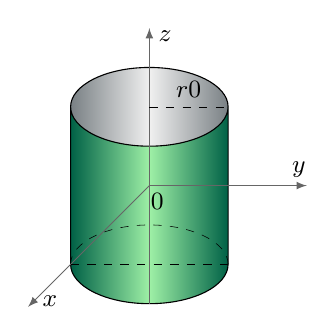
\begin{tikzpicture}
  \usetikzlibrary{arrows}
  \definecolor{insideo}{HTML}{798084}
  \definecolor{insidei}{HTML}{F0F0F0}
  \definecolor{outer}{HTML}{006146}
  \definecolor{inner}{HTML}{9EF0A6}
  \shade [left color=insideo,right color=insideo,middle color=insidei] (1,1) arc (0:180:1 and .5) --
   (-1,1) arc (180:360:1 and .5);
  \shadedraw [left color=outer,right color=outer,middle color=inner] (-1,-1) arc (180:360:1 and .5) -- (1,1) --
   (1,1) arc (360:180:1 and .5) -- (-1,-1);
  \draw (1,1) arc (0:180:1 and .5);
  \draw [dashed,line width=0.2pt] (1,-1) arc (0:180:1 and .5);
  \draw [black!60,line width=0.3pt,-latex] (0,0) -- (2,0,0);
  \draw [black!60,line width=0.3pt,-latex] (0,-1.5) -- (0,2,0);
  \draw [black!60,line width=0.3pt,-latex] (0,0) -- (0,0,4);
  \pgfputat{\pgfpointxyz{1.9}{0.2}{0}}{\pgfbox[center,center]{\small $y$}};
  \pgfputat{\pgfpointxyz{0.2}{1.9}{0}}{\pgfbox[center,center]{\small $z$}};
  \pgfputat{\pgfpointxyz{0.2}{0}{3.8}}{\pgfbox[center,center]{\small $x$}};
  \pgfputat{\pgfpointxyz{0.1}{-0.2}{0}}{\pgfbox[center,center]{\small $0$}};
  \draw [dashed,line width=0.2pt] (0,1) -- (1,1);
  \draw [dashed,line width=0.2pt] (-1,-1) -- (1,-1);
  \node [above] at (0.5,1) {\small $\ssub{r}{0}$};
 \end{tikzpicture}}
 \qquad\qquad
 \subfloat[][$\theta = \ssub{\theta}{0}$]{
 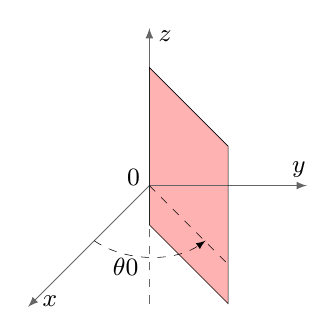
\begin{tikzpicture}
  \usetikzlibrary{arrows}
  \fill [red!30] (0,-.5) -- (1,-1.5) -- (1,.5) -- (0,1.5) -- (0,-.5);
  \draw [black!60,line width=0.3pt,-latex] (0,0) -- (2,0,0);
  \draw [black!60,line width=0.3pt,-latex] (0,-.5) -- (0,2,0);
  \draw [black!60,dashed,line width=0.3pt] (0,-1.5) -- (0,-.5);
  \draw [black!60,line width=0.3pt,-latex] (0,0) -- (0,0,4);
  \pgfputat{\pgfpointxyz{1.9}{0.2}{0}}{\pgfbox[center,center]{\small $y$}};
  \pgfputat{\pgfpointxyz{0.2}{1.9}{0}}{\pgfbox[center,center]{\small $z$}};
  \pgfputat{\pgfpointxyz{0.2}{0}{3.8}}{\pgfbox[center,center]{\small $x$}};
  \pgfputat{\pgfpointxyz{-0.2}{0.1}{0}}{\pgfbox[center,center]{\small $0$}};
  \draw [line width=0.2pt] (0,-.5) -- (1,-1.5) -- (1,.5) -- (0,1.5) -- (0,-.5);
  \draw [dashed,line width=0.2pt] (0,0) -- (1,-1);
  \draw [dashed,line width=0.2pt,-latex] (-0.7,-0.7) arc (225:315:1 and .7);
  \node [below] at (-0.3,-.8) {\small $\ssub{\theta}{0}$};
 \end{tikzpicture}}
 \qquad\qquad
 \subfloat[][$z = \ssub{z}{0}$]{
 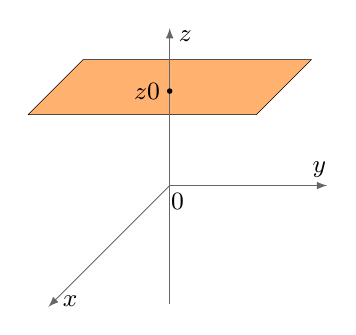
\begin{tikzpicture}
  \usetikzlibrary{arrows}
  \definecolor{planecolor}{HTML}{FFB270}
  \fill [planecolor] (-1.8,.9) -- (-1.1,1.6) -- (1.8,1.6) -- (1.1,.9) -- (-1.8,.9);
  \draw [line width=0.2pt] (-1.8,.9) -- (-1.1,1.6) -- (1.8,1.6) -- (1.1,.9) -- (-1.8,.9);
  \draw [black!60,line width=0.3pt,-latex] (0,0) -- (2,0,0);
  \draw [black!60,line width=0.3pt,-latex] (0,-1.5) -- (0,2,0);
  \draw [black!60,line width=0.3pt,-latex] (0,0) -- (0,0,4);
  \pgfputat{\pgfpointxyz{1.9}{0.2}{0}}{\pgfbox[center,center]{\small $y$}};
  \pgfputat{\pgfpointxyz{0.2}{1.9}{0}}{\pgfbox[center,center]{\small $z$}};
  \pgfputat{\pgfpointxyz{0.2}{0}{3.8}}{\pgfbox[center,center]{\small $x$}};
  \pgfputat{\pgfpointxyz{0.1}{-0.2}{0}}{\pgfbox[center,center]{\small $0$}};
  \fill (0,1.2) circle (1pt);
  \node [left] at (0,1.2) {\small $\ssub{z}{0}$};
 \end{tikzpicture}}
 \caption[]{\quad Cylindrical coordinate surfaces}
 \label{fig:cylcoordsurf}
\end{figure}

The unit vectors $\hat r, \hat \theta,\hat k$ at any point $P$ are perpendicular to the surfaces $r =$ constant, $\theta =$ constant, $z =$ constant
 through $P$ in the directions of increasing $r, \theta, z$. Note that the direction of the unit vectors $\hat r,\hat \theta$ vary from point to point, unlike the corresponding Cartesian unit vectors.




\begin{center}
\tdplotsetmaincoords{70}{120}
\begin{tikzpicture}[tdplot_main_coords,scale=0.7]
\tikzstyle{every node}=[font=\small]
\filldraw[fill=Maroon, fill opacity=0.3] (-4,-4,4) -- (4,-4,4) --  (4,5,4) -- (-4,5,4) -- (-4,-4,4);
\filldraw[fill=RoyalBlue, nearly transparent] (0,0,4) -- (5.2,6,4) --  (5.2,6,0) -- (0,0,0) -- (0,0,4);
\draw[-latex] (0,0,0) -- (6,0,0) node[anchor=north east]{$x$};
\draw[-latex] (0,0,0) -- (0,6,0) node[anchor=north west]{$y$};
\draw[-latex] (0,0,0) -- (0,0,6) node[anchor=south]{$z$};
\draw (0,0,0) circle (3);
\draw (0,0,4) circle (3);
\draw (1.9,-2.35,0) -- (1.9,-2.35,4) node[midway, left]{$r=r_1$ surface};
\draw (-1.9,2.35,0) -- (-1.9,2.35,4);
\filldraw [color=blue!30](2,2.25,4) circle (0.075cm) ;
\draw (-4,5,4) node[anchor=south]{$z=z_1$ plane};
\draw (5.2,6,0) node[anchor=south west]{$\phi=\phi_1$ plane};
\node at (2.05,.7,4)  { $P_1(r_1,\phi_1,z_1)$};
\draw[ thick,-latex](2,2.25,4) -- (3,3.45,4) node[anchor=north] {$\hat r$};
\draw[ thick,-latex](2,2.25,4) -- (1,2.5,4) node[anchor=north west] {$\hat \phi$};
\draw[ thick,-latex](2,2.25,4) -- (2,2.25,4.75) node[anchor=north west] {$\hat k$};
\draw [thick,->](4,0,0) arc (0:45:4 and 4.5);
\draw (3.6,2,0) node[anchor=north] {$\phi_1$};
\draw[ thick,-latex](0,0,0) -- (2,2.35,0);
\draw (1,1,0) node[anchor=north] {$r_1$};
\draw [ thick] (2,2.25,4)--(1.95,2.25,0);
\draw[ thick](0.1,0,4) -- (-0.1,0,4) node[anchor=south west] {$z_1$};
\end{tikzpicture}
\end{center}




For spherical coordinates $(\rho,\theta,\phi)$, and constants $\ssub{\rho}{0}$, $\ssub{\theta}{0}$ and $\ssub{\phi}{0}$,
we see from Figure \ref{fig:sphcoordsurf}
that the surface $\rho = \ssub{\rho}{0}$ is a sphere of radius $\ssub{\rho}{0}$ centered at the origin, the surface
$\theta = \ssub{\theta}{0}$ is a half-plane emanating from the $z$-axis, and the surface $\phi = \ssub{\phi}{0}$ is a
circular cone whose vertex is at the origin.

\begin{figure}[h]
 \centering
 \subfloat[][$\rho = \ssub{\rho}{0}$]{
 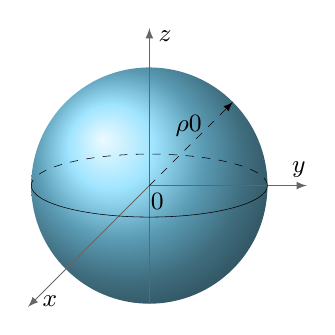
\begin{tikzpicture}
  \usetikzlibrary{arrows}
  \definecolor{spherecolor}{HTML}{80DCFF}
  \shade [ball color=spherecolor] (0,0) circle (1.5);
  \draw [black!60,line width=0.3pt,-latex] (0,0) -- (2,0,0);
  \draw [black!60,line width=0.3pt,-latex] (0,-1.5) -- (0,2,0);
  \draw [black!60,line width=0.3pt,-latex] (0,0) -- (0,0,4);
  \pgfputat{\pgfpointxyz{1.9}{0.2}{0}}{\pgfbox[center,center]{\small $y$}};
  \pgfputat{\pgfpointxyz{0.2}{1.9}{0}}{\pgfbox[center,center]{\small $z$}};
  \pgfputat{\pgfpointxyz{0.2}{0}{3.8}}{\pgfbox[center,center]{\small $x$}};
  \pgfputat{\pgfpointxyz{0.1}{-0.2}{0}}{\pgfbox[center,center]{\small $0$}};
  \draw [line width=0.2pt] (-1.5,0) arc (180:360:1.5 and 0.4);
  \draw [dashed,line width=0.2pt] (1.5,0) arc (0:180:1.5 and 0.4);
  \draw [dashed,line width=0.2pt,-latex] (0,0) -- (1.06,1.06);
  \node [above] at (0.5,0.5) {\small $\ssub{\rho}{0}$};
 \end{tikzpicture}}
 \qquad\qquad
 \subfloat[][$\theta = \ssub{\theta}{0}$]{
 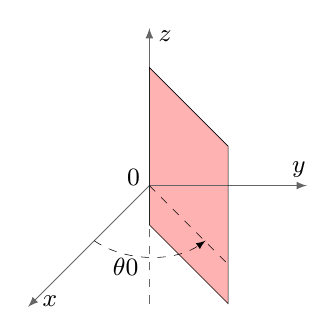
\begin{tikzpicture}
  \usetikzlibrary{arrows}
  \fill [red!30] (0,-.5) -- (1,-1.5) -- (1,.5) -- (0,1.5) -- (0,-.5);
  \draw [black!60,line width=0.3pt,-latex] (0,0) -- (2,0,0);
  \draw [black!60,line width=0.3pt,-latex] (0,-.5) -- (0,2,0);
  \draw [black!60,dashed,line width=0.3pt] (0,-1.5) -- (0,-.5);
  \draw [black!60,line width=0.3pt,-latex] (0,0) -- (0,0,4);
  \pgfputat{\pgfpointxyz{1.9}{0.2}{0}}{\pgfbox[center,center]{\small $y$}};
  \pgfputat{\pgfpointxyz{0.2}{1.9}{0}}{\pgfbox[center,center]{\small $z$}};
  \pgfputat{\pgfpointxyz{0.2}{0}{3.8}}{\pgfbox[center,center]{\small $x$}};
  \pgfputat{\pgfpointxyz{-0.2}{0.1}{0}}{\pgfbox[center,center]{\small $0$}};
  \draw [line width=0.2pt] (0,-.5) -- (1,-1.5) -- (1,.5) -- (0,1.5) -- (0,-.5);
  \draw [dashed,line width=0.2pt] (0,0) -- (1,-1);
  \draw [dashed,line width=0.2pt,-latex] (-0.7,-0.7) arc (225:315:1 and .7);
  \node [below] at (-0.3,-.8) {\small $\ssub{\theta}{0}$};
 \end{tikzpicture}}
 \qquad\qquad
 \subfloat[][$\phi = \ssub{\phi}{0}$]{
 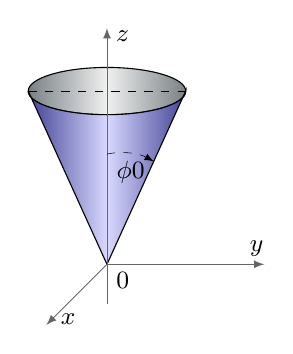
\begin{tikzpicture}
  \usetikzlibrary{arrows}
  \definecolor{insideo}{HTML}{798084}
  \definecolor{insidei}{HTML}{F0F0F0}
  \definecolor{outer}{HTML}{424296}
  \definecolor{inner}{HTML}{D8D8FF}
  \shadedraw [left color=insideo,right color=insideo,middle color=insidei] (1,2.2) arc (0:180:1 and .3) --
   (-1,2.2) arc (180:360:1 and .3);
  \shadedraw [left color=outer,right color=outer,middle color=inner] (-1,2.2) arc (180:360:1 and .3) -- (0,0) --
   (-1,2.2);
  \draw [black!60,line width=0.3pt,-latex] (0,0) -- (2,0,0);
  \draw [black!60,line width=0.3pt,-latex] (0,-.5) -- (0,3,0);
  \draw [black!60,line width=0.3pt,-latex] (0,0) -- (0,0,2);
  \pgfputat{\pgfpointxyz{1.9}{0.2}{0}}{\pgfbox[center,center]{\small $y$}};
  \pgfputat{\pgfpointxyz{0.2}{2.9}{0}}{\pgfbox[center,center]{\small $z$}};
  \pgfputat{\pgfpointxyz{0.2}{0}{1.8}}{\pgfbox[center,center]{\small $x$}};
  \pgfputat{\pgfpointxyz{0.2}{-0.2}{0}}{\pgfbox[center,center]{\small $0$}};
  \draw [dashed,line width=0.2pt] (-1,2.2) -- (1,2.2);
  \draw [dashed,line width=0.2pt,-latex] (0,1.4) arc (100:65:1 and 1.2);
  \node [above] at (0.3,0.9) {\small $\ssub{\phi}{0}$};
 \end{tikzpicture}}
 \caption[]{\quad Spherical coordinate surfaces}
 \label{fig:sphcoordsurf}
\end{figure}

Figures \ref{fig:cylcoordsurf}(a) and \ref{fig:sphcoordsurf}(a) show how these coordinate systems got their names.

Sometimes the equation of a surface in Cartesian coordinates can be transformed into a simpler equation in some other
coordinate system, as in the following example.

\vspace{2mm}
     \begin{exa}
 Write the equation of the cylinder $x^2 + y^2 = 4$ in cylindrical coordinates.\vspace{1mm}
\end{exa}
 \begin{solu}
Since $r = \sqrt{x^2 + y^2}$, then the equation in cylindrical
 coordinates is $r =2$.
 \end{solu}
 
  

Using spherical coordinates to write the equation of a sphere does not necessarily make the
equation simpler, if the sphere is not centered at the origin.

\vspace{2mm}
     \begin{exa}
 Write the equation $(x - 2)^2 + (y - 1)^2 + z^2 = 9$ in spherical coordinates.\vspace{1mm}
\end{exa}

\begin{solu}
Multiplying the equation out gives
 \begin{align*}
  x^2 + y^2 + z^2 - 4x - 2y + 5 &= 9 \text{~, so we get}\\
  \rho^2 - 4 \rho \sin \phi \,\cos \theta - 2 \rho \sin \phi \,\sin \theta - 4 &= 0 \text{~,~or}\\
  \rho^2 - 2 \sin \phi \, ( 2 \cos \theta - \sin \theta \, ) \,\rho - 4 &= 0
 \end{align*}
 after combining terms. Note that this actually makes it more difficult to figure out what the surface is,
 as opposed to the Cartesian equation where you could immediately identify the surface as a sphere of radius $3$ centered
 at $(2,1,0)$.
\end{solu}


     \begin{exa}\label{exa:helicoid}
 Describe the surface given by $\theta = z$ in cylindrical coordinates.
\end{exa}

\begin{solu}
 This surface is called a \emph{helicoid}\index{helicoid}. As the (vertical) $z$
 coordinate increases, so does the angle $\theta$, while the radius $r$ is unrestricted. So this sweeps out a (ruled!)
 surface shaped like a spiral staircase, where the spiral has an infinite radius. Figure \ref{fig:helicoid} shows a
 section of this surface restricted to $0 \le z \le 4\pi$ and $0 \le r \le 2$.
\end{solu}


 \begin{figure}[h]
  \begin{center}
   \includegraphics[width=7cm]{./figs/Helicoid}
  \end{center}\vspace{-12mm}
 \caption[]{\quad Helicoid $\theta = z$}
 \label{fig:helicoid}
 \end{figure}
\vspace{0.5cm}       
       
\section*{\psframebox{Exercises}}
\probs{A}
\par\noindent For Exercises 1-4, find the (a) cylindrical and (b) spherical coordinates of the point whose
Cartesian coordinates are given.
\begin{enumerate}
 \begin{multicols}{2}
  \item $(2,2\sqrt{3},-1)$
  \item $(-5,5,6)$
  \item $(\sqrt{21},-\sqrt{7},0)$
  \item $(0,\sqrt{2},2)$
 \end{multicols}
\suspend{enumerate}
\par\noindent For Exercises 5-7, write the given equation in (a) cylindrical and (b) spherical coordinates.
\resume{enumerate}[{}]
 \begin{multicols}{2}
  \item $x^2 + y^2 + z^2 = 25$
  \item $x^2 + y^2 = 2y$
  \item $x^2 + y^2 + 9z^2 = 36$
 \end{multicols}
\suspend{enumerate}
\probs{B}\vspace{1mm}
\resume{enumerate}[{}]
 \item Describe the intersection of the surfaces whose equations in spherical coordinates are $\theta = \dfrac{\pi}{2}$
  and $\phi = \dfrac{\pi}{4}$.
 \item Show that for $a \ne 0$, the equation $\rho = 2a \sin \phi \, \cos \theta$ in spherical coordinates describes a
  sphere centered at $(a,0,0)$ with radius $\abs{a}$.
\suspend{enumerate}
\probs{C}
\resume{enumerate}[{}]
 \item Let $P = (a,\theta,\phi)$ be a point in spherical coordinates, with $a > 0$ and $0 < \phi < \pi$. Then $P$ lies
  on the sphere $\rho = a$. Since $0 < \phi < \pi$, the line segment from the origin to $P$
  can be extended to intersect the cylinder given by $r = a$ (in cylindrical coordinates). Find the cylindrical
  coordinates of that point of intersection.
 \item Let $\ssub{P}{1}$ and $\ssub{P}{2}$ be points whose spherical coordinates are
  $( \ssub{\rho}{1},\ssub{\theta}{1},\ssub{\phi}{1} )$ and $( \ssub{\rho}{2},\ssub{\theta}{2},\ssub{\phi}{2} )$,
  respectively. Let $\ssub{\textbf{v}}{1}$ be the vector from the origin to $\ssub{P}{1}$, and let
  $\ssub{\textbf{v}}{2}$ be the vector from the origin to $\ssub{P}{2}$. For the angle $\gamma$ between
%   $\ssub{\textbf{v}}{1}$ and $\ssub{\textbf{v}}{2}$, show that
  \begin{displaymath}
   \cos \gamma = \cos \ssub{\phi}{1} \, \cos \ssub{\phi}{2} + \sin \ssub{\phi}{1} \, \sin \ssub{\phi}{2} \,
    \cos ( \, \ssub{\theta}{2} - \ssub{\theta}{1} \, ) .
  \end{displaymath}
  This formula is used in electrodynamics to prove the addition theorem for spherical harmonics, which provides a
  general expression for the electrostatic potential at a point due to a unit charge. See pp. 100-102 in \cite{jac}.
 \item Show that the distance $d$ between the points $\ssub{P}{1}$ and $\ssub{P}{2}$ with cylindrical coordinates
  $( \ssub{r}{1},\ssub{\theta}{1},\ssub{z}{1} )$ and $( \ssub{r}{2},\ssub{\theta}{2},\ssub{z}{2} )$, respectively, is
  \begin{displaymath}
   d = \sqrt{\ssub{r}{1}^2 + \ssub{r}{2}^2 - 2 \ssub{r}{1}\,\ssub{r}{2} \cos (\, \ssub{\theta}{2} - \ssub{\theta}{1} \,)
   + ( \ssub{z}{2} - \ssub{z}{1} )^2} \, .
  \end{displaymath}
 \item Show that the distance $d$ between the points $\ssub{P}{1}$ and $\ssub{P}{2}$ with spherical coordinates
  $( \ssub{\rho}{1},\ssub{\theta}{1},\ssub{\phi}{1} )$ and $( \ssub{\rho}{2},\ssub{\theta}{2},\ssub{\phi}{2} )$,
  respectively, is
  \begin{displaymath}
   d = \sqrt{\ssub{\rho}{1}^2 + \ssub{\rho}{2}^2 - 2 \ssub{\rho}{1}\,\ssub{\rho}{2} [ \sin \ssub{\phi}{1} \,
    \sin \ssub{\phi}{2} \,\cos ( \, \ssub{\theta}{2} - \ssub{\theta}{1} \, ) +
    \cos \ssub{\phi}{1} \, \cos \ssub{\phi}{2} ]} \, .
  \end{displaymath}
\end{enumerate}


\section{$\star$ Cross Product in the n-Dimensional Space}

In this section we will answer the following question: Can one define a cross product in the n-dimensional space so that it will have properties similar to the usual 3 dimensional one?

Clearly the answer depends which properties we require.


The most direct
generalizations of the cross product are to define either:

\begin{itemize} 
\item a binary product $\times :\bbR^n\times \bbR^n \to \bbR^n$ which takes as input two vectors and
  gives as output a vector;
\item
  a $n-1$-ary product $\times :\underbrace{\bbR^n\times \dots \times  \bbR^n}_{n-1 \text{ times}}  \to \bbR^n$  which takes as input
  \(n-1\) vectors, and gives as output one  vector.
\end{itemize}

Under the correct assumptions it can be proved that a binary product exists only in the dimensions 3 and 7. A simple proof of this fact can be found in \cite{mcloughlin2012does}.

In this section we focus in the definition of the $n-1$-ary product. 


\begin{df} Let $\vector{v}_1,\dots,\vector{v}_{n-1}$ be vectors in
\(\mathbf{R}^n,\), and let  $\lambda \in
\reals$ be a scalar. Then we  define their generalized cross product
\( \vector{v}_{n} = \vector{v}_1 \times \cdots \times \vector{v}_{n-1}\) as the \( (n-1)\)-ary product satisfying
\begin{dingautolist}{202}
\item {\textbf  Anti-commutativity:} 
$\vector{v}_1 \times \cdots \vector{v}_i \times \vector{v}_{i+1}  \times \dots \times  \vector{v}_{n-1}= -
\vector{v}_1 \times \cdots \vector{v}_{i+1} \times \vector{v}_{i}  \times \dots \times  \vector{v}_{n-1}$,
i.e, changing two consecutive vectors a minus sign appears.
\item {\textbf
Bilinearity:} 
$\vector{v}_1 \times \cdots \vector{v}_i+\vector{x} \times \vector{v}_{i+1}  \times \dots \times  \vector{v}_{n-1}
=\vector{v}_1 \times \cdots \vector{v}_i \times \vector{v}_{i+1}  \times \dots \times  \vector{v}_{n-1} +
\vector{v}_1 \times \cdots \vector{x} \times \vector{v}_{i+1}  \times \dots \times  \vector{v}_{n-1}$

\item {\textbf  Scalar homogeneity:}
$\vector{v}_1 \times \cdots \lambda \vector{v}_i \times \vector{v}_{i+1}  \times \dots \times  \vector{v}_{n-1}
=\lambda \vector{v}_1 \times \cdots \vector{v}_i \times \vector{v}_{i+1}  \times \dots \times  \vector{v}_{n-1}$

\item {\textbf  Right-hand Rule:}
\( \vector{e}_{1} \times \cdots \times \vector{e}_{n-1} = \vector{e}_n\),
\( \vector{e}_{2} \times \cdots \times \vector{e}_n = \vector{e}_{1},\) and so forth for
cyclic permutations of indices.

\end{dingautolist}
\end{df}

We will also write 
\[\bigtimes(\vector{v}_1,\dots,\vector{v}_{n-1}):=\vector{v}_1 \times \cdots \vector{v}_i \times \vector{v}_{i+1}  \times \dots \times  \vector{v}_{n-1}  \]




In coordinates, one can give a formula for this
\( (n-1)\)-ary analogue of the cross product in
$\bbR^n$ by:

\begin{prop} 
Let   $\vector{e}_1,\dots,\vector{e}_{n}$ be the canonical basis of \(\mathbf{R}^n\) and 
let $\vector{v}_1,\dots,\vector{v}_{n-1}$ be vectors in
\(\mathbf{R}^n,\) with coordinates:
\begin{eqnarray*}
 \vector{v}_1&=&(v_{11}, \dots v_{1n})\\
&\vdots&\\
 \vector{v}_i&=&(v_{i1}, \dots v_{in})\\
&\vdots&\\
 \vector{v}_n&=&(v_{n1}, \dots v_{nn})\\
\end{eqnarray*}
in the canonical basis.  Then 

\[\bigtimes(\vector{v}_1,\dots,\vector{v}_{n-1}) =
  \begin{vmatrix}
 v_{11} &\cdots &v_{1n}\\
    \vdots  &\ddots &\vdots\\
    v_{n-1 1} & \cdots &v_{n-1 n}\\
    \mathbf{e}_1 &\cdots &\mathbf{e}_{n}
  \end{vmatrix}.\]  
\end{prop}  

This formula is very similar  to the determinant formula for
the normal cross product in $\bbR^3$ except that
the row of basis vectors is the last row in the determinant rather than
the first.

The reason for this is to ensure that the ordered vectors
\[(\vector{v}_1, ...,\vector{v}_{n-1},
\bigtimes(\vector{v}_1,
...,\vector{v}_{n-1}))\]
have a positive orientation with respect to
\[(\vector{e}_1, ..., \vector{e}_n).\]

\begin{prop} 
\begin{dingautolist}{202} The vector product have the following properties:
\item The vector $\bigtimes(\vector{v}_1,\dots,\vector{v}_{n-1})$ is 
  perpendicular to  \( \vector{v}_{i},\)
\item
 the  magnitude of $\bigtimes(\vector{v}_1,\dots,\vector{v}_{n-1})$ is the volume of the solid  defined by the vectors
\( \vector{v}_{1}, \dots \vector{v}_{i-1}\)
\item 
$\vector{v}_n\bp  \vector{v}_{1} \times \cdots \times \vector{v}_{n-1} =
  \begin{vmatrix}
    v_{11} &\cdots &v_{1n}\\
    \vdots  &\ddots &\vdots\\
    v_{n-1 1} & \cdots &v_{n-1 n}\\
    v_{n1} &\cdots &v_{n1}
  \end{vmatrix}.$
\end{dingautolist}  
\end{prop}



\section{Multivariable Functions}
Let $A\subseteq \reals^n$. For most of this course, our concern will
be functions of the form
$$f:A \subseteq \reals^n \to \reals^m.  $$If $m=1$, we say that $f$ is a 
\negrito{scalar
field}. If $m\geq 2$, we say that $f$ is a \negrito{vector field}.




We would like to develop a calculus analogous to the situation in
$\reals$. In particular, we would like to examine limits,
continuity, differentiability, and integrability of multivariable
functions. Needless to say, the introduction of more variables
greatly complicates the analysis. For example, recall that the graph
of a function $f:A\rightarrow \reals^m$, $A\subseteq \reals^n$.  is
the set
$$ \{(\point{x},f(\point{x})): \point{x}\in A)\}\subseteq \reals^{n+m}. $$
If $m+n>3$, we have an object of more than three-dimensions! In the case $n=2, m=1$, we have a tri-dimensional surface.
We will now briefly examine this case.

\begin{df}
Let $A\subseteq \reals^2$ and let $f:A\to \reals$ be a function.
Given $c\in\reals$, the \negrito{level curve} at $z=c$ is the curve
resulting from the intersection of the surface $z=f(x,y)$ and the
plane $z=c$, if there is such a curve.
\end{df}



\begin{exa}
The level curves of the surface $f(x,y)=x^2+3y^2$ (an elliptic paraboloid) are the concentric ellipses
$$x^2+3y^2 = c,  \qquad c>0. $$
\end{exa}
\begin{figure}[h]
 \centering
 \includegraphics[width=6cm]{./figs/contour1.eps}
 % contour1.eps: 0x0 pixel, 300dpi, 0.00x0.00 cm, bb=
 \caption{Level curves for $f(x,y)=x^2+3y^2$.}
 \label{fig:contour}
\end{figure}




\subsection{Graphical Representation of Vector Fields}

In this section we present a graphical representation of vector fields. 
For this intent, we limit ourselves to low dimensional spaces.

A vector field $\vector{v}:\bbR^3\to \bbR^3$ is an assignment of a vector  $\vector{v} = \vector{v}(x , y , z)$  
to each point $(x , y , z)$ of a subset $U\subset \bbR^3$. Each vector $\vector{v}$ of the field can be regarded
as a "bound vector" attached to the corresponding point $( x , y , z)$.  In components
\[\vector{v}(x,y,z)=v_1(x,y,z)\vector{i}+v_2(x,y,z)\vector{j}+v_3(x,y,z)\vector{k}.\]


\begin{exa}
 Sketch each of the following vector fields.
 \item $\vector{F}=x\vector{i}+y\vector{j}$
 \item $\vector{F}=-y\vector{i}+x\vector{j}$
 \item $ \mathbf r = x\vector{i} + y \vector{j} + z\vector{k}$
\end{exa}

\begin{solu}

a) The vector field is null at the origin; at other points, $\vector{F}$
is a vector pointing away from the origin;

b) This vector field is perpendicular to the first one at every point;

c) The vector field is null at the origin; at other points, $\vector{F}$
is a vector pointing away from the origin. This is the $3$-dimensional 
analogous of the first one.
\end{solu}



\begin{figure}[h]
 \centering
 \includegraphics[width=4.5cm]{./figs/vectorf1.eps}
  \includegraphics[width=4.5cm]{./figs/vectorf2.eps}
\scalebox{0.8}{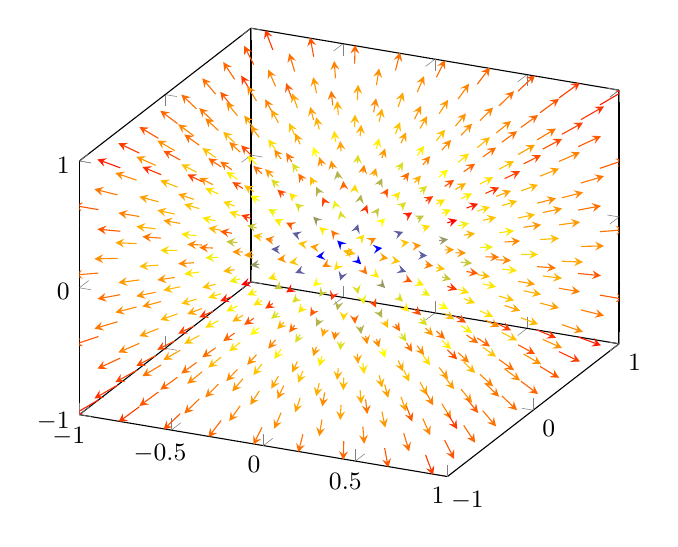
\begin{tikzpicture}
  \begin{axis}[
    domain=-1:1,
    samples=10,
    xmin=-1,xmax=1,
    ymin=-1,ymax=1,
    zmin=-1,zmax=1,
    ]
    \pgfplotsinvokeforeach{-1,-.5,0,.5,1}{
      \addplot3[cyan,quiver,-stealth,
      point meta={sqrt((x)^2+(y)^2+(z)^2)},
      quiver={
        u={x},
        v={y)},
        w={z},
        colored,scale arrows=.1}]
      (x,y,#1);
    }
  \end{axis}
\end{tikzpicture}}


 % vectorf1.eps: 0x0 pixel, 300dpi, 0.00x0.00 cm, bb=
\end{figure}


\begin{exa}
Suppose that an object  of mass $M$ is located at
the origin of a three-dimensional coordinate system. We can think of this object as
inducing a force field $\funvect{g}$ in space. The effect of this gravitational field is to attract any
object placed in the vicinity of the origin toward it with a force that is governed by Newton's Law of Gravitation. 
\[\funvect{F}=\dfrac{GmM}{r^2}\]

To find an expression for $\funvect{g}$ , suppose that an object of mass $m$ is
located at a point  with position vector $r= x\vector{i} + y\vector{j} + z\vector{k}$ . 

The gravitational field is the gravitational force exerted per unit mass on a small test mass (that won't distort the field) at a point in the field. Like force, it is a vector quantity: a point mass M at the origin produces the gravitational field
\[\funvect{g} = \funvect{g}(\vector{r}) = -\dfrac{GM}{r^{3} }\vector{r},\]
where $\vector{r}$ is the position relative to the origin and where $r=\norm{\vector{r}}$. Its magnitude is
\[g=-\dfrac{GM}{r^{2} }\]
and, due to the minus sign, at each point $\funvect{g}$ is directed opposite to $\vector{r}$, i.e. towards the central mass.
\end{exa}

\begin{figure}[h]
 \centering
 \includegraphics[width=6cm]{./figs/vectfield-potencial.eps}
 % vectfield-potencial.eps: 0x0 pixel, 300dpi, 0.00x0.00 cm, bb=
 \caption{Gravitational Field}
 \label{fig:gravfield}
\end{figure}




\section*{\psframebox{Exercises}}
\begin{multicols}{2}\columnseprule 1pt \columnsep 25pt\multicoltolerance=900

\begin{problem}
Sketch the level curves for the following maps.
\begin{enumerate}
\item $(x,y)\mapsto x+y$
\item $(x,y)\mapsto xy$
\item $(x,y)\mapsto \min (|x|,|y|)$
\item $(x,y)\mapsto x^3-x$
\item $(x,y)\mapsto x^2+4y^2$
\item $(x,y)\mapsto \sin (x^2+y^2)$
\item $(x,y)\mapsto \cos (x^2-y^2)$
\end{enumerate}
\end{problem}
\begin{problem}
Sketch the level surfaces for the following maps.
\begin{enumerate}
\item $(x,y,z)\mapsto x+y+z$
\item $(x,y,z)\mapsto xyz$
\item $(x,y,z)\mapsto \min (|x|,|y|, |z|)$
\item $(x,y,z)\mapsto x^2+y^2$
\item $(x,y,z)\mapsto x^2+4y^2$
\item $(x,y,z)\mapsto \sin (z-x^2-y^2)$
\item $(x,y,z)\mapsto x^2+y^2+z^2$
\end{enumerate}
\end{problem}



\end{multicols}


\section{Levi-Civitta and Einstein Index Notation}





We need an efficient abbreviated notation to handle the complexity of mathematical structure before us. We will use indices of a given ``type" to denote all possible values of given index ranges. By index type we mean a collection of similar letter types, like those from the beginning or middle of the Latin alphabet, or Greek letters
\begin{eqnarray}
&& a,b,c,\ldots
\nonumber\\
&& i,j,k,\ldots
\nonumber\\
&& \lambda,\beta,\gamma\ldots
\nonumber
\end{eqnarray}
each index of which is understood to have a given common range of successive integer values.
Variations of these might be barred or primed letters or capital letters.
For example, suppose we are looking at linear transformations between ${\mathbb R}^n$ and ${\mathbb R}^m$ where $m\ne n$. We would need two different index ranges to denote vector components in the two vector spaces of different dimensions, say 
$i,j,k,...=1,2,\ldots,n$  and $\lambda,\beta,\gamma,\ldots=1,2,\ldots,m$.

In order to introduce the so called Einstein summation convention, we agree to the following limitations on how indices may appear in formulas.
A given index letter may occur only once in a given term in an expression (call this a ``free index"), in which case the expression is understood to stand for the set of all such expressions for which the index assumes its allowed values, or  it may occur twice but only as a superscript-subscript pair (one up, one down) which will stand for the sum over all allowed values (call this a ``repeated index"). Here are some examples. If $i,j=1,\ldots,n$ then

\medskip
$A^i \longleftrightarrow 
n\ {\textrm expressions}: A^1,A^2,\ldots,A^n$,

$A^i{}_{i}\longleftrightarrow 
\dsum_{i=1}^n A^i{}_{i}$, a single expression with $n$ terms \\
\null\hskip 1 in 
(this is called the trace of the matrix $\underline{A}=(A^i{}_j)$),

$A^{ji}{}_{i}\longleftrightarrow 
\dsum_{i=1}^n A^{1i}{}_{i},\ldots, \dsum_{i=1}^n A^{ni}{}_{i}$, $n$ expressions each of which has $n$ terms in the sum, 	
 
$A_{ii}\longleftrightarrow$ no sum, just an expression for each $i$, if we want to refer to a specific
\\ $\phantom{A_{ii}\longleftrightarrow {\quad }}$\ \
 diagonal component (entry) of a matrix, for example,

$A^i v_i + A^i w_i = A^i(v_i+w_i)$, 
 2 sums of $n$ terms each (left) or one combined sum (right).
\medskip

A repeated index is a ``dummy index," like the dummy variable in a definite integral
\[\dint^b_a f(x)\dx=\dint^b_a f(u)\du.\]		
We can change them at will: $A^i{}_i=A^j{}_j$.



\begin{rem}
In order to emphasize that we are using Einstein's convention, we
will enclose any terms under consideration with \es{\cdot}.
\end{rem}
\begin{exa}
Using Einstein's Summation convention, the dot product of two
vectors $\vector{x}\in\reals^n$ and $\vector{y}\in\reals^n$ can be
written as
$$ \dotprod{x}{y} =\sum _{i=1} ^n x_iy_i = \es{x_ty_t}.$$
\end{exa}
\begin{exa}
Given that $a_i, b_j, c_k, d_l$ are the components of vectors in
$\reals^3$, $\vector{x}, \vector{y},  \vector{z}, \vector{d}$
respectively, what is the meaning of $$\es{a_ib_ic_kd_k} ?
$$
\end{exa}
\begin{solu}
We have
$$\es{a_ib_ic_kd_k}  = \sum _{i=1} ^3 a_ib_i\es{c_kd_k} = \dotprod{x}{y}\es{c_kd_k} = \dotprod{x}{y}\sum _{k=1} ^3 c_kd_k = (\dotprod{x}{y})(\dotprod{c}{d}).  $$
\end{solu}

\begin{exa}
Using Einstein's Summation convention, the  $ij$-th entry
$(AB)_{ij}$ of the product of two matrices $A\in\mat{m\times
n}{\reals}$ and $B\in\mat{n\times r}{\reals}$ can be written as
$$ (AB)_{ij} = \sum _{k=1} ^n A_{ik}B_{kj}=    \es{A_{it}B_{tj}}.$$
\end{exa}
\begin{exa}
Using Einstein's Summation convention, the trace $\tr{A}$ of a
square matrix $A\in\mat{n\times n}{\reals}$  is  $\tr{A}= \sum
_{t=1} ^n A_{tt}=\es{A_{tt}}$.
\end{exa}
\begin{exa}
Demonstrate, via Einstein's Summation convention, that if $A, B$ are
two $n\times n$ matrices, then $$ \tr{AB}=\tr{BA}. $$
\end{exa}
\begin{solu}
We have
$$ \tr{AB}  = \tr{(AB)_{ij}}=\tr{\es{A_{ik}B_{kj}}} =\es{\es{A_{tk}B_{kt}}},  $$
and
$$ \tr{BA}  = \tr{(BA)_{ij}}=\tr{\es{B_{ik}A_{kj}}} =\es{\es{B_{tk}A_{kt}}}, $$
from where the assertion follows, since the indices are dummy
variables and can be exchanged.
\end{solu}

\begin{df}[Kroenecker's Delta] The symbol $\delta
_{ij}$ is defined as follows:
$$ \delta _{ij} = \left\{ \begin{array}{ll} 0 & \mathrm{if}\ i\neq j \\
1 & \mathrm{if}\ i = j.
\end{array}
\right.
$$
\end{df}
\begin{exa}
It is easy to see that $\es{\delta _{ik}\delta _{kj}} = \sum _{k=1}
^3 \delta _{ik}\delta _{kj}=\delta _{ij}$.
\end{exa}
\begin{exa}
We see that $$\es{\delta _{ij}a_ib_j} = \sum _{i=1} ^3 \sum _{j=1}
^3\delta _{ij}a_ib_j = \sum _{k=1} a_kb_k = \dotprod{x}{y}.
$$
\end{exa}
Recall that a \negrito{permutation} of distinct objects is a reordering
of them. The $3!=6$ permutations of the index set  $\{1,2,3\}$ can
be classified into \negrito{even} or \negrito{odd}. We start with the
identity permutation $123$ and say it is even. Now, for any other
permutation, we will say that it is even if it takes an even number
of transpositions (switching only two elements in one move) to
regain the identity permutation, and odd if it takes an odd number
of transpositions to regain the identity permutation. Since
$$ 231 \to 132 \to 123, \quad 312 \to 132 \to 123, $$the
permutations $123$ (identity), $231$, and $312$ are even. Since
$$ 132 \to 123, \quad  321 \to 123, \quad 213 \to 123, $$the
permutations $132$, $321$, and $213$ are odd.

\begin{df}[Levi-Civitta's Alternating Tensor] The symbol $\varepsilon
_{jkl}$ is defined as follows:
$$ \varepsilon _{jkl} = \left\{ \begin{array}{ll} 0 & \mathrm{if}\ \{j,k,l\} \neq \{1,2,3\} \\
-1 & \mathrm{if}\ \begin{pmatrix} 1 & 2 & 3 \\ j & k & l \\
\end{pmatrix}\ \mathrm{is\ an \ odd\ permutation }\\
+1 & \mathrm{if}\ \begin{pmatrix} 1 & 2 & 3 \\ j & k & l \\
\end{pmatrix}\ \mathrm{is\ an \ even\ permutation }\\
\end{array}
\right.
$$
\end{df}
\begin{rem}
In particular, if one subindex is repeated we have $\varepsilon
_{rrs}=\varepsilon _{rsr}=\varepsilon _{srr}=0$. Also,
$$ \varepsilon
_{123}= \varepsilon _{231}=\varepsilon _{312}=1, \qquad  \varepsilon
_{132}= \varepsilon _{321}=\varepsilon _{213}=-1.$$

\end{rem}


\begin{exa}
Using the Levi-Civitta alternating tensor and Einstein's summation
convention, the cross product can also be expressed, if
$\vector{i}=\vector{e_1}$, $\vector{j}=\vector{e_2}$,
$\vector{k}=\vector{e_3}$, then
$$\crossprod{x}{y} = \es{\varepsilon _{jkl}(a_kb_l)\vector{e_j}}.$$
\end{exa}
\begin{exa}
If $A=[a_{ij}]$ is a $3\times 3$ matrix, then, using the
Levi-Civitta alternating tensor,
$$\det A = \es{\varepsilon _{ijk}a_{1i}a_{2j}a_{3k}}.  $$
\end{exa}
\begin{exa}
Let $\vector{x}, \vector{y}, \vector{z}$ be vectors in $\reals^3$.
Then $$ \vector{x}\bp (\crossprod{y}{z}) =
\es{x_i(\crossprod{y}{z})_i} = \es{x_i\varepsilon _{ikl}(y_kz_l) }.
$$
\end{exa}

\section*{\psframebox{Exercises}}\begin{multicols}{2}\columnseprule 1pt \columnsep 25pt\multicoltolerance=900
\begin{problem}
Let $\vector{x}, \vector{y}, \vector{z}$ be vectors in $\reals^3$.
Demonstrate that
$$  \es{x_iy_iz_j} = (\dotprod{x}{y})\vector{z}. $$
\end{problem}
\end{multicols}

